\documentclass[12pt]{article}
\usepackage{natbib}
\usepackage{graphicx}
\usepackage{array} 
\usepackage{mathtools}
\usepackage{amsmath}
\usepackage{amssymb}
\usepackage{multirow}
\usepackage{subfig}
\usepackage{tikz}
\usetikzlibrary{calc}
\usetikzlibrary{decorations.pathreplacing}
\usetikzlibrary{matrix,shapes.geometric}
\usepackage[font=small,labelfont=bf]{caption}
\usepackage[letterpaper,top=2cm,bottom=2cm,left=3cm,right=3cm,marginparwidth=2cm]{geometry}
\linespread{1.4}
\setlength{\bibsep}{0pt plus 0.3ex}

\bibliographystyle{apalike}
\title{Systemic Risk and Financial Connectedness: Empirical Evidence}
\author{Mateusz Dadej}
\date{\today}

\begin{document}

\maketitle

\section{Introduction}

A fundamental characteristic that distinguishes systemic events from idiosyncratic ones are the relation between the system participants. A common sequence of a systemic contagion, is when a supposedly firm specific events becomes transmitted into the cross-sectional dimension. Clearly, the way particular entities are interacting within the system is a key characteristic in order to understand the dynamics and severity of systemic events. This is what separates the common approach to systemic risk, where the stability of the system is but a sum of idiosyncratic risks, to the one that emphasizes the role of system structure. These contrasting distinctions are best captured by the concepts of \textit{too-big-to-fail} and \textit{too-interconnected-to-fail}. Where the former, emphasizes the sheer size of the entity and its potential impact on the system in case of default. On the other hand, the latter term describes the way the system depends on that particular institution, due to its central role within the system. It has been acknowledged that the macroprudential policy was too focused on the sheer size of institutions, but insufficiently on their systemic contribution (see e.g. \cite{bernanke09} or \cite{rajan09}). That being said, it is crucial to view the system through the lenses of both of these approaches, for they are complimentary when assessing the stability of the financial system.

This approach to the systemic risk, gave a rise to the concept of \textit{robust yet fragile} property of the financial system. In the context of financial markets, the term was first coined\footnote{Before that, the term was commonly used in the complexity science (see e.g. \cite{doyle05} and \cite{carlson02})} by the economist at the Bank of England, Andrew Haldane (\cite{haldane13}). He posits, that due to its interconnectedness, the financial system exhibits a tipping point property. The connections among financial institutions serves as a shock absorbers, as long as the extent of the shock is limited. The common links allow for a shock to be spread throughout the network, at the same time suppressing the damages of the initial shock. However, once the extent of the shock exceeds a certain point, the properties of the contagion changes markedly. The network of the institutions no longer works as shock absorber, but as a shock amplifier of the initial disturbance. The damages are transmitted further on, disturbing the banks in a chain reaction. With the final contagion substantially exceeding the degree of the initial shock. The contagion is transmitted akin to the spread of the disease. 

A relatively new strain of literature, that incorporates the way institutions are forming the financial networks, have emerged as a response to the increasing connections among the market participants. The literature provides several theoretical models describing the aforementioned property\footnote{In fact, the \textit{robust yet fragile} property of the financial system was described before it was called as such (see e.g \cite{gai10}, first published in 2008, or \cite{gallegati08}).}. One of the extension of the property is described in \cite{acemoglu13}. They provide a simple, yet profound model in which a more densely connected financial network improves the stability of the system when faced by a shock, relatively smaller in magnitude. On the other hand, similarly to the \textit{robust yet fragile} property, beyond some degree of the shock, more dense connections of the system are undermining the stability thereof. Thus, their conjecture highlights, that the network density may have a substantially different effect depending on which regime the markets currently are. 

Considering the above theoretical literature, herein work aims at providing an empirical evidence to the regime-dependent effect of the network density on the stability of the financial system. We mostly follow the description of the \textit{robust yet fragile} property as in \cite{acemoglu13}, however, the evidence is easily applicable to the other models (see \cite{glasserman16} for an extensive literature review). To the best knowledge of the authors, there has not been a study that provides an empirical evidence of this phenomenon.

More precisely, our research design is a two-step process. First, we collect a time series of stock prices of the systematically important banks in both US and EU. Based on the data, we estimate the network between the banks and its density in a rolling window basis. In order to achieve robust results, the modeling approach is based on several methods, well established in the literature of network econometrics. This procedure results in a time series of financial connectedness for the particular financial market. In the second step, we estimate a Markov switching ARCH model, where the connectedness is the exogenous, regime-dependent variable. We assume, that a volatility of particular banking index reflects the stability thereof. Additionally, we provide a series of robustness checks, \textit{inter alia}, by including the financial statement data of the banks in the modeling framework.

The model endogenously finds two distinct regimes of the analyzed relationship. The results indeed provide an evidence confirming the set of theoretical models. The effect of the network density on the stability of the financial system varies depending on the regimes. However, the effect is much asymmetrical. During the stable market regime, the network density has almost no effect on the stability of the financial system. At the same time, more dense financial network, is undermining the stability of the system during the unstable market regime\footnote{\cite{acemoglu13} describe these regimes as "small shock" and "large shock" respectively.}. It is, thus, evident that the increased bank interconnectedness is in total a damaging property of the financial markets. 

The remainder of the paper is structured as follows. Next section provides a brief literature review and its link to herein paper. Section.......

\section{Literature}\label{section:literature}

As the research aims at connecting the theoretical models of the financial networks with the empirical evidence, the relevant literature is divided into theoretical and empirical part.

One of the earliest seminal models describing the contagion through the lens of financial networks was \cite{allen00}. Where they arrive to the very intuitive conclusion that a complete network\footnote{In graph theory, a complete graph has connections among all of its nodes.} between the banks, is more robust to the contagion than the incomplete one. The mechanism is that the more diversified network of banks allows the liquidity shock to spread among the network. A similar conclusion can be drawn from the work of \cite{freixas00}, where they emphasize the role of the central bank in coordinating the banking system during the contagion. An important advancement in analyzing financial networks was introduced in \cite{eisenberg01}. They provide a method to obtain a clearing vector among the banks, that clears their obligation. Additionally, they prove uniqueness of the vector. The method is extensively used for modeling the contagion in the financial networks and has been extended, e.g. for liquidity consideration (\cite{cifuentes05}) or for liquidation costs (\cite{rogers13}). 

Since the first works, modeling banking system as a financial network, there was an increased effort into describing alternative ways of contagion propagation in this framework. One of the very first ones was described in \cite{cifuentes05}, where the banks are interconnected through common market asset holdings. They show, that when the market's demand for illiquid assets is not perfectly elastic, selling them on the market by the banks may decrease prices substantially. At the same time, due to mark-to-market accounting, other banks with the same holdings may be under pressure to sell their assets, further depressing and generating the fire sales. This contagion may begin even from lesser shocks. \citet{elliot14} emphasize the role of bankruptcy cost in amplifying the cascading effect of the contagion. Their model also distinguishes integration from the network connectedness, defining it as a degree of dependence from the network. They show, that although integration can increase the likelihood of a cascade once an initial failure happens, it might also decrease the chance of that first failure. \cite{caballero13} shows, that once the contagion begin, the banks are facing an increasingly complex environment as they need to monitor the bigger part of the network in order to control their own default risk. This uncertainty induced counterparty risk causes precautionary behavior among banks, further exacerbating the fire sale.

A considerably more relevant strain of literature to herein research considers the nonlinear effect of the connectedness on contagion dynamics. Based on previously studied concept of percolation on random graph from complexity science (\cite{callaway00} or \cite{newman001}), \cite{gai10} show that the financial system exhibits a similar form of phase transition. Specifically, due to the dense structure of the financial networks, the likelihood of contagion is particularly low. However, the same property makes the contagion very severe once it happens. Based on the same model, \cite{may10} apply mean-field approximation, to identify the contribution of various parameters in the model to the likelihood and severity of the contagion. An already mentioned research of \cite{acemoglu13}, goes beyond the model of \cite{gai10}. They suggest, that the degree of connectedness of the financial system have a regime-dependent effect on stability, at the same time proving the narrative of Andrew Haldane (\cite{haldane13}). The contribution of herein research is exactly to provide an empirical evidence of their work as well as the intuition of policymakers.  

Since the work is mostly empirical in nature, it is also imperative to position it among the literature of network econometrics. Although scarce in data, there has been several works statistically describing the actual transaction level data\footnote{The data is often proprietary to the public entities regulating the financial markets.} and thus, the network among the banks.  Using Bundesbank data on bilateral interbank exposures among 2000 banks from 1999 to 2012, \cite{craig14} provide evidence for tiering on the interbank market. The banks are forming a very hierarchical network, where a lower-tiered banks are interacting between each other mostly through the intermediating banks, mostly bigger in size\footnote{A similar behavior is also present in other economic networks e.g. international trade (\cite{antras11})}. The tiering behavior is modeled and commonly referred to in the literature as a \textit{core-periphery} structure. Based on the Italian interbank market data from January 1999 to December 2010, \cite{fricke2015} confirm previous contribution, at the same time showing, that the core of the financial network is highly persistent in time. That is, the banks forming the core don't change the position in the structure. \cite{langfield14} extend the previous research with the data across other class of assets held among the banks (such as derivatives, marketable securities, repo, unsecured lending and secured lending). They emphasize particular heterogeneity of the financial network, by distinguishing between interbank funding and interbank exposures. The structure is significantly different among these types, thus the dynamics of contagion varies depending on the source of risk (liquidity vs. credit risk). Clearly, the contribution of this part of the literature is mostly in describing the stylized facts present in the actual financial networks.

As much as the network data is available (although to the very limited extent), the econometricians aimed at estimating the financial networks from broadly available sources, mostly from equity price time series. \cite{billio12} describe a pair of econometric methods, that are employed as part of this work. They use monthly stock prices of insurers, hedge funds and banks to estimate their interconnectedness. In the first approach they suggest a model based on principal component analysis (Hereafter referred to as PCA, \cite{murihead09}). When used on the covariance matrix of stock returns, the PCA will provide a set of factors eigenvalues best describing the variation of the system. A higher share of the variance, explained by top eigenvalues, indicates elevated connectedness in the system. A second model provides more detailed information by estimating a whole directed network of the financial institutions. The method is based on the "Granger causality" (\cite{granger69}) among the pair of allegedly connected entities. The financial network is constructed by performing the granger test on each of pairs of the stock returns with adjacency matrix entries being one or zero depending on the outcome of the test. The resulting approach allows higher flexibility in analyzing the topology of the network and deciding the measures of connectedness (the authors use a range of different network measures). These methods are employed in the research design and more closely described later on. 

Alternative methodology to estimate financial networks from the stock prices data was developed by \cite{deibold14}. In their work, the financial network\footnote{Or in the paper's terminology - a connectedness table.} is estimated as a matrix of parameters from the Vector Autoregression model (\cite{sims80}). Precisely, the adjacency matrix of the network is the $\Theta$ from the VAR matrix notation: $\boldsymbol{y}_t = \theta_o + \boldsymbol{\Theta} \boldsymbol{y}_{t-1} + \epsilon_t$. In a similar vein to \cite{billio12}, the authors use their method to estimate the network and appropriate connectedness measures among the financial institutions from USA\footnote{The same approach was applied also to other data. For example, international trade (\cite{deibold23}) commodities (\cite{diebold17} and \cite{gong22}), cryptocurrencies (\cite{ji19}), particular pair of countries (\cite{dadej23})  and among the whole asset classes (\cite{bouri21}).}. As these methods may seems to be substitutable at first, the authors themselves point out the differences between their approach and that of \cite{billio12}. Considering the VAR methodology, it is evident that the resulting network of connections is weighted, unlike the Granger-based approach. This provide another dimension to analyze the strength of the links among the institutions. Moreover, at least in the standard formulation, the Granger-based approach is only pairwise. That is, it does not control for the spurious relationship, stemming from the confounding third (or more, in that matter) entity. However, the Granger-based method is flexible enough to extend the main regression used to test the Granger causality by more control variables. There are, of course, some disadvantages to rely on the VAR approach. It requires identifying assumptions, related to the variance decomposition. Also, what is more relevant to the herein research is higher computational burden coming from the VAR approach. Given, that the research design does not require information on link weights and is computationally expensive, the approach of \cite{billio12} was considered to be more appropriate.

There is a number of alternative methods used for estimating networks in general, but more often used in other fields of study. A common approach from systems biology are Gaussian graphical models (e.g. applied in \cite{friedman04}). They allow for maximum likelihood estimation with penalization, producing a robust network estimation. Some of the applications in finance were estimating international finance flows (\cite{giudici16}) or systemic risk on the banking sector (\cite{cerchiello16}). \cite{barigozzi19} employs common approach to estimate network with VAR, but they extend the methodology with LASSO estimation (\cite{breiman95}), allowing for sparsity of the network and improved forecasting.

Another strain of literature, suggesting the methods to estimate financial networks, comes from a different data source. Banks do not provide counterparty information in their financial statements but they do show their aggregated values for both lending and borrowing on the interbank market. This is a source of hard data that provides the marginal values for the adjacency matrix of the network, i.e. the columns and rows sums. Several authors provided methods of filling the adjacency matrix at the same time satisfying some stylized facts regarding financial networks. The stylized facts are provided by the research based on the actual data (surveyed before in herein section) or commonly accepted economic rationale, in case of no self-lending restriction. One of the most common approach is to estimate the network as evenly as possible. This method, know as \textit{maximum entropy} (\cite{upper11}), assumes that banks are trying to diversify their holdings as much as possible. The supposition that banks are diversifying as much as possible, may seems appealing at first. However, due to the monitoring costs and informal relationships (\cite{brauning16}) among banks (\cite{cocco09}), it is not realistic. Most likely overestimating density of the actual financial network. Having that in mind, \cite{anand15} suggest a \textit{minimum density} method which minimizes the total number of linkages necessary for allocating interbank positions. An appealing characteristic of the method is that it is overestimating the degree of contagion (according to the author's comparison). This is contrary to the benchmark methods, which more often underestimate it. A method suggested by \cite{baral12}, draws a link weights based on the copula distribution fitted to the aggregated interbank data. \cite{cimini15} uses fitness model based on likelihood  of directed connections with additional knowledge of the node's parameters. \citet{drehmann13} takes into account a commonly recognized stylized fact regarding the interbank market, that the network exhibits a \textit{core-periphery} structure. Their method provides a reconstructed matrix with \textit{core-periphery} characteristic. \cite{halaj13} suggest an iterative method were the network links are drawn randomly until the network is reconstructed. Above methods are compared together in a horse race described in \cite{anand18}.

A literature considering connections between financial institutions in the context of systemic risk and contagion is vast. Considering the increased importance of connectedness for assessing the systemic risk, \cite{hautsch14} improve on the works of \cite{adrian16} to propose the realized systemic risk beta. The measure specify the contribution of particular financial institution to the systemic risk, given its position in the network. A similar metric is suggested by \cite{dungey12}. They rank financial institutions in order of their systemic importance, considering their correlation-based connectedness. \cite{savona14} estimate dynamic conditional correlation model, in order to study the contagion among the hedge funds. The author shows, that correlations are key factor for predicting depressed hedge fund returns. A broader perspective is shown in the work of \cite{minoiu15}. According to their research, an elevated country connectedness, and at the same time, decrease in those of its neighbors, is able to predict the banking crisis.

\section{Data}\label{section:Data}

The main set of results is based on the equity stock prices and indices data. The stock data is adjusted for corporate actions such as splits and dividends. The analysis focus on the data of financial institutions from two biggest financial sectors. Namely, that of United States and European Union. An exact list of the institutions follows the stress test exercises from both of the banking sectors analyzed (\cite{eba2021} and \cite{fed21}). The number of institutions is 31 and 42 for USA and EU respectively. The full list is presented in the table \ref{table:bank_list} in the appendix \ref{appendix:data}. Not every company was listed from the beginning of the analyzed period. The list of the first available price data (thus including in the analysis) is presented in table \ref{table:ipo} in the appendix \ref{appendix:data}. Additionally, the relevant banking indices are used as a proxy of financial stability (KBW Nasdaq Bank Index and EURO STOXX® Banks) and broad market indices for control (S\&P500 and STOXX® Europe 600). A robustness check incorporates financial statements of the institutions into analysis. The financial variables are obtained from Orbis database for each quarter between 2017Q3 and 2024Q4\footnote{However, due to missing reports for some institutions the actual data used is smaller}. The source of the data is Yahoo Finance. 

\subsection{Summary statistics}\label{subsection:data_descrptive}

Table \ref{table:descriptive} reports descriptive statistics of the stock price data for both of the markets. On average the stock prices have a (slight) upward trend with average return being positive and similar for both of the markets. Although, once the sample is split pre and post Great Financial Crisis (hereafter referred to as GFC), there are substantial differences. The average returns are higher post-GFC for USA than before, au contraire, the European returns were higher pre-GFC. It clearly shows, the banking dimension of the debt crisis that hit the Europe in the second decade of 21st century. It is also evident that the European market is more volatile. Every dispersion measure is higher for EU than USA. This is as expected, considering the more severe banking crises in a lot of European member states (e.g. Greece, Italy and Ireland). Unlike in the USA, where there was no substantial banking contagion after the 2008 subprime crisis. 

% latex table generated in R 4.3.2 by xtable 1.8-4 package
% Sat Jul 20 20:45:35 2024
\begin{table}[h]
	\centering
	\begin{tabular}{r|r|r}
		market & EU & USA \\ 
		\hline \hline
		Average return (\%)& 0.0395 & 0.0412 \\ 
		Std. deviation (\%)& 3.83 & 2.49 \\ 
		max drawdown (\%)& -88.77 & -83.17 \\
		1\% percentile (\%)& -7.55 & -6.63 \\ 
		99\% percentile (\%)& 7.76 & 6.99 \\ 
		worst return (\%)& -93.33 & -59.03 \\ 
		max return (\%)& 1400 &   86.9 \\ 
		Average correlation & 0.398 & 0.617 \\
		Sample size & 5748 & 5844 \\ 
	\end{tabular}
	\caption{Descriptive statistics of the data. The statistics are averages over stock returns and markets. In case of maximum and minmium values, the minimum (for stocks) of the minimum (for each market) and vice versa for the maximum.}
	\label{table:descriptive}
\end{table}


The American market is on average more correlated than the European one. The reason is more fragmented banking sector\footnote{Although, the concept of Banking union is discussed.} in Europe, with different member states having a separate banking law, regulators, capital markets and in general a more heterogeneous real economy. That being said, the systemic risk of the banking sector is indeed a EU-wide concern (see e.g. \cite{song21}). 


\section{Financial network connectedness}\label{section:fin_network}

Because of lack of public data from the interbank market, or as a matter of fact, any bilateral contractual obligations between the banks, the academic literature developed a set of tools to estimate the financial networks from available sources. As shown in the literature, these methods are well established and commonly applied in order to estimate the financial connections. This is despite some of their limitations. One may wonder, how can the stock prices reflect an information that is not public? There is however, evidence, that the stock prices discount also some unknown information to the public, e.g. due to insider trading or inferred from other data. A classic example is \cite{newhard14}, describing the, allegedly, the first ever event study performed on the stock prices. Based on the outperformance of lithium producers he inferred the fuel material used in the manufacturing of the newly-developed hydrogen bomb. An information which was non-public, to the extent, that his paper was confiscated. The literature on insider trading and non-public information on the stock market is vast and extends beyond the scope of herein paper (see e.g. \cite{hawk90}, \cite{huddart07} or \cite{klein20}). As well as assessment of the methods to estimate the financial network.

A schematic representation describing the problem faced by both \cite{billio12} and \cite{diebold17} of financial network estimation is shown in the Figure \ref{fig:connectedness_scheme}. Based on the multivariate time-series data matrix $X$, consisting of stock price returns, the authors suggest a method of inferring an adjacency matrix, describing the connections among the financial institutions. As shown, the adjacency matrix has a number of columns and rows equal to the number of entities. Each of the elements in the adjacency matrix $\boldsymbol{A}$, describe the connections between the entities. That is, $a_{i,j} > 0 \Rightarrow i \rightarrow j \; \forall \;  i \neq j$. In the economic applications, the diagonal values are usually zero, as there is no intuition behind a self connection of a financial institution. Each $a_{i,j}$ can take binary values in case of unweighted graph or any other real-valued number in case of weighted graph. A very useful property, linking linear algebra and graph theory is that every graph has its own adjacency matrix (and vice versa). Thus, a variety of graph theory measures may be applied to the estimated network of connections. One of the most common measure describing the financial connectedness is the average degree, which is average number of edges each of the graph nodes has. The measure may provide a single value number describing the connectedness of entirety of financial system (at least so far as goes the number of included financial institutions). 

\begin{figure}
	\begin{tikzpicture}	
		% Matrix
		\begin{scope}[scale = 0.9, xshift=0.5]
			\matrix (m) [matrix of math nodes,left delimiter=(,right delimiter=),ampersand replacement=\&] {
				x_{11} \& x_{12} \& \dots \& x_{1n} \\
				x_{21} \& x_{22} \& \dots \& x_{2n} \\
				x_{31} \& x_{32} \& \dots \& x_{3n} \\
				\vdots \& \vdots \& \ddots \& \vdots \\
				x_{T1} \& x_{T2} \& \dots \& x_{Tn} \\
			};
			
			\draw [decorate,decoration={brace,amplitude=10pt}]
			(2.6,-1.8) -- (-2.6,-1.8) node [black,midway,xshift=0cm,yshift=-0.7cm] 
			{\footnotesize Time series matrix $\boldsymbol{X}$ of size $T \times n$.};
		\end{scope}
		
		\begin{scope}[scale= 0.6]
			\draw[->, line width = 0.7] (5,0) -- (8,0) node[midway, above] {\footnotesize $f: \mathbb{R}^{T\times n}\to \mathbb{R}^{n \times n}$};
		\end{scope}
		
		\begin{scope}[scale = 0.9, xshift = 8.5cm]
			\matrix (m) [matrix of math nodes,left delimiter=(,right delimiter=),ampersand replacement=\&] {
				a_{11} \& a_{12} \& \dots \& a_{1n} \\
				a_{21} \& a_{22} \& \dots \& a_{2n} \\
				\vdots \& \vdots \& \ddots \& \vdots \\
				a_{n1} \& a_{n2} \& \dots \& a_{nn} \\
			};
			
			\draw[decorate,decoration={brace,amplitude=10pt}]
			(2.6,-1.6) -- (-2.6,-1.6) node [black,midway,yshift=-0.9cm] 
			{\footnotesize Adjacency matrix $\boldsymbol{A} \times n$.};
		\end{scope}
		
		\draw[line width=1pt] (7.5,-2.9) -- (7.5,-3.4);
		\draw[line width=1pt] (7.35,-2.9) -- (7.35,-3.4);
		
		% Pentagram graph
		\begin{scope}[xshift=7.5cm, yshift = -5.5cm, scale=0.8]
			\node[draw, circle, inner sep=1pt] (a) at (90:1.8) {$x_p$};
			\node[draw, circle, inner sep=1pt] (b) at (162:2) {$x_1$};
			\node[draw, circle, inner sep=1pt] (c) at (234:2) {$x_2$};
			\node[draw, circle, inner sep=1pt] (d) at (306:2) {$x_3$};
			\node[draw, circle, inner sep=1pt] (e) at (18:2) {$x_4$};
			
			\draw[<->] (a) -- (c);
			\draw[<->] (c) -- (e);
			\draw[<->] (e) -- (b);
			\draw[<->] (b) -- (d);
			\draw[<->] (d) -- (a);
			
			\draw[<->] (a) -- (b);
			\draw[<->] (b) -- (c);
			\draw[<->] (c) -- (d);
			\draw[<->] (d) -- (e);
			\node[xshift=1.9, yshift=2.1, scale=1.1] at ($(e)!.5!(a)$) {$\ddots$};
			%\draw[dotted, <->] (e) -- (a);
			
			\draw [decorate,decoration={brace,amplitude=10pt}]
			(2,-2) -- (-2,-2) node [black,midway, yshift=-0.6cm] 
			{\footnotesize Graph representation of matrix $\boldsymbol{A}$.};
			
		\end{scope}
	\end{tikzpicture}
	\caption{Scheme describing the process of financial network estimation.}
	\label{fig:connectedness_scheme}
\end{figure}



In what follows in the section, the particular methods of estimating the financial networks are described. Out of the three methods employed in the research design, the last two of the them follows the work of \cite{billio12}. With the first one suggested by the author. 

\subsection{Ledoit-Wolf covariance}\label{subsection:ledoit_wolf}

This approach follows a commonly applied in finance (and in portfolio optimization in particular) shrinkage method suggested by \cite{ledoit03}.The idea behind shrinkage is to compute the convex linear combination of sample covariance $\hat{\Sigma} = \frac{1}{N}\boldsymbol{X}'\boldsymbol{X}$ (with elements $\hat{\sigma}_{i,j}$) of rates of returns matrix $\boldsymbol{X}$ and an identity matrix $\mathbb{I}$:

\begin{equation}
	\tilde{\Sigma} \coloneqq \rho_1 \mathbb{I} + \rho_2 \hat{\Sigma}
\end{equation}

The optimal linear combination above is the solution to the following quadratic program subject to linear constraint:

\begin{equation}
	\begin{aligned}
	\max_{\rho_1, \rho_2} \quad &  \mathbb{E}[|| \tilde{\Sigma} - \Sigma||^2] \\
	\textrm{s.t.} \quad & \tilde{\Sigma} = \rho_1 \mathbb{I} + \rho_2 \hat{\Sigma}
	\end{aligned}
\end{equation}

Where the $||\cdot||$ is the Frobenius norm defined\footnote{For the purpose of this exercise, this is a slightly modified version of the Frobenius norm.} as $||A|| = \sqrt{\frac{1}{N} \sum_{i=1}^{N} \sum_{j=1}^{N} a_{i,j}^2}$. With solution equal to:

\begin{equation}
	\tilde{\Sigma} = \frac{\beta^2}{\delta^2} \mu \mathbb{I} + \frac{\alpha^2}{\delta^2} \hat{\Sigma}
\end{equation}

The estimators of $\beta^2$, $\delta^2$, $\alpha^2$ and $\mu$ being:

\begin{equation}
	\begin{aligned}
	\hat{\mu}_T = \frac{1}{N} \sum_{i=1}^{N} \sigma^T_{i,i} \\
	\hat{\delta}^2_T = ||\hat{\Sigma}_T - \hat{\mu}_T \mathbb{I}_T ||^2 \\
	\hat{\beta}^2_T = \min \left\{ \frac{1}{T} \sum_{t=1}^T || x_t^T (x_t^T)' - \hat{\Sigma}_T||^2,\, \hat{\delta}^2_T \right\}
	\end{aligned}
\end{equation}

Once the shrinked covariance matrix is estimated, it is assumed to reflect the underlying connections among the financial institutions. The connectedness is thus measured as an average Ledoit-Wolf covariance among the entities:

\begin{equation}
	\gamma_{lw} = \frac{\sum_{i \neq j}^{N} \sum_{j \neq i}^N \tilde{\sigma}_{i,j}}{N^2 - N}
\end{equation}

Where $\tilde{\sigma}_{i,j}$ are, as before, elements of the matrix $\tilde{\Sigma}$.

The procedure tends to pull the most extreme parameters into more central values, thus systematically reducing estimation error. The estimation error is especially substantial when the dimension of the analyzed data is high, with respect to the amount of observations available. another work by the original authors \cite{ledoit04} performs a Monte Carlo simulation study benchmarking alternative ways to estimate the covariance matrix and shows the superiority of their approach for large dimensional data. This is considerably relevant considering research design of this work. As mentioned before, the connectedness measure will be calculated in a rolling window basis. Often as small as a single quarter (63 observations vs. 42 variables). 

\subsection{Principal component analysis}\label{subsection:pca}

A connectedness measure based on the principal component analysis (PCA) is the first method suggested by \cite{billio12}. The idea is to calculate the share of variance explained by the top $k$ component. In principle, the PCA is the eigendecomposition of a covariance matrix (with variance of covariates scaled to one). Namely, we wish to find an eigenvector $\nu$ and eigenvalue $\lambda$ that satisfy following equation:

\begin{equation}
	\hat{\Sigma} \mathbf{v} = \lambda \mathbf{v}
\end{equation}

The values of interest may be find solving a homogeneous system of
linear equations $|\hat{\Sigma} - \lambda \mathbb{I}| = 0$, with $|\cdot|$ being a determinant operator. An important property of the eigenvectors is their orthogonality. The covariance matrix is decomposed in a following way:

\begin{equation}
	\hat{\Sigma} = \mathbf{Q}\mathbf{\Lambda}\mathbf{Q}'
\end{equation}

Where $\mathbf{\Lambda} = \text{diag} \{\lambda_1, \lambda_2, \dots, \lambda_n \}$ and $\mathbf{Q}$ is an orthogonal matrix whose columns are unit eigenvectors. Thus, the eigendecomposition yields a set of uncorrelated components fully explaining (linearly) the underlying covariance matrix. The eigenvalues reflect the variance explained by the relative eigenvector.

In the context of the data used in this research, the biggest eigenvalue shows the amount of variance of the returns, explained by the most important factor. Thus, the relevant measure of the connectedness is:

\begin{equation}
	\gamma_{pca} = \frac{\max \{\mathbf{\lambda}\}}{\mathbf{\lambda}'\mathbf{1}}
\end{equation}

Where $\mathbf{1}$ is a vector of ones with appropriate size. The measure may be interpreted as a share of the single most important component in explaining the total sum of the variances. It is clear, that the measure have some drawbacks when analyzing connectedness. The procedure does not yield the connections among the institutions (other than covariance itself) but a single measure of connectedness. Notwithstanding this disadvantage, the measure is useful in the context of herein research design, as the main objective of this stage is to obtain the single connectedness measure. 

\subsection{Granger based connectedness measure}\label{subsection:granger}

The approach, that yields not only a network of the connections but also its directionality is based on the concept of Granger causality (\cite{granger69}). The variable $x_t$ is said to "Granger-cause" a variable $y_t$ if it contains enough information at time $t-1$ to predict the respective variable in the next period $t$. Naturally, this statement is tested by running a regression with lagged variable:

\begin{equation}\label{equation:granger}
	y_t = \beta_0 + \beta_1 x_t + \underbrace{\sum_{i=1}^{p} \beta_{i+1} y_{t - p}}_{\text{lag controls}} + \epsilon_t
\end{equation}

Where $\beta$ are the estimated coefficients and $\epsilon_t$ the uncorrelated error term. The variable $x_t$ is said to Granger-cause $y_t$ if the respective coefficient $\beta_1$ is significantly different from zero.
In the context of financial markets, the above approach may appear to be implausible to a lot of financial economists. That is because of the relatively high degree of information efficiency, considering we analyze the most liquid markets in the world. This efficiency implies that any publicly accessible information should yield no predictive ability, thus rendering the equation \ref{equation:granger} pointless. That being said, the test indeed finds the underlying connections \footnote{Even with a frequency higher than the applied confidence interval.}. This is due to several factors. The primary one, is that the statistical significance is not equal to the economical one. Any execution of potential strategy following the equation \ref{equation:granger}, will stumble upon the transaction costs, including slippage and commissions, which will make the exercise unprofitable. Thus, the granger causality may just as well be seen as a return spillover between the institutions, as shown in \cite{battison12}.

The exact procedure employed in the research design is slightly modified\footnote{\cite{billio12} performs the Granger causality test by filtering the returns with GARCH(1,1) process and then using the time-varying variance to test the significance of the $\beta$ coefficient from the regression. This approach is, however, computationally more expensive. This technical dimension is more relevant to this study as the connectedness is measured in a rolling window basis. Unlike in the original study of \cite{billio12}.}. The procedures uses excess returns of the institutions stock prices over a relevant benchmark of market rates of return. Consequently, the returns of the institutions will have a purely idiosyncratic character. The regression has a following specification:

\begin{equation}
	r_{i,t+1} = \beta_0 + \beta_1 r_{j,t} + \beta_2 r_{i, t} + \underbrace{\sum_{i=1}^{k} \beta_{i+2} x_{t}}_{\text{Sectoral controls}} + \epsilon_t
\end{equation}

The financial institutions are assumed to be connected when the $\beta_1$ coefficient is statistically different from 0. The sectoral controls consists of rates of returns of consumer discretionary ETF, Real Estate ETF, crude oil WTI and treasure bills of 3-month and 10 year maturity. These variables control for common shocks among the institutions. Since the institutions may have a common exposures (e.g. to real estate through mortgages portfolio), a shock to the real estate market could hit both of the institutions equally, showing potential Granger causality, despite no bilateral contractual obligations among them. By introducing some of the sectoral controls the research design is free from this sort of relationship. It is however important to note, that these channels are also of concern by the theoretical literature studying contagion on the financial networks. This channel is described e.g. by \cite{cifuentes05} and may play an actual role in the mechanism describing the \textit{robust-yet-fragile} phenomena. That being said, this is one of the three other methods estimating the financial connectedness in herein study and the only one where controlling for the common shock is possible. Thus, the other measures will be allowed to capture this channel. 

The above Granger analysis is ran on every pair of the institutions. The adjacency matrix of the financial network $\boldsymbol{A}$ has following entries:

\begin{equation}
	a_{i,j} = \begin{cases}
		1  & \text{if } \beta_1 \text{ is significant} \\
		0 & \text{otherwise}
	\end{cases} \; \forall \; i \neq j
\end{equation}

Thus, the resulting graph is unweighted, because the adjacency matrix is binary. Although, this is only a matter of choice. The entries might as well be equal to the effect size $\beta_1$. This is however unnecessary, given the research design. Since the Granger causality is not granted, the network is also directed. Clearly, these properties of the approach are beneficial with respect to the rest employed. The method is also different in a way that it measures the lagged connection among the entities. It is unclear if that is the most suitable approach, considering that the information is discounted in real time on the financial markets. 

The connectedness measure is then calculated in a similar manner as for the Ledoit-Wolf approach:

\begin{equation}
\gamma_{g} = \frac{\sum_{i \neq j}^{N} \sum_{j \neq i}^N a_{i,j}}{N^2 - N}	
\end{equation}

\section{Network estimation results}\label{section:network_results}

\subsection{Static analysis}\label{subsection:static}

Although, the ground truth of the true financial network is unknown, it is still informative to investigate the properties of the estimated networks. This way we can evaluate if the estimation results are economically sensible. Figure \ref{fig:actual_network} shows two representations of the same graph, estimated with the Granger-based method. The data used for the estimation is from 2023, as the actual links among the financial institutions is concentrated within this horizon\footnote{The data on maturity structure on interbank market is scarce as well. A bit outdated but complete sample from the German interbank market from 2000 reports that around 40\% of the interbank debt has a maturity of less than a year (\cite{upper04}). The inclusion of derivatives would most likely increase this share.}. It is clear from the visual presentation of the network, how dense the connection is\footnote{The definition of \textit{density} as well as other network statistics used in this section and henceforth is described in the appendix \ref{appendix:network_metrics}}. As reported in the table \ref{table:network_metrics}, the visualized graph is more dense than for the USA market and different time periods. The European financial sector is less densely connected than the USA, in both of the period subsample. This is to be expected (also from the descriptive statistics in the subsection \ref{subsection:data_descrptive}), considering that the banking sector is more fragmented due to separate jurisdictions. In absolute terms, every estimated network is somewhat more dense \footnote{This is, however, arbitrary to some degree. The level of density might be as well manipulated by choosing different confidence level when checking the $\beta$ coefficient significance in Granger test. Increasing its level from 95\% to e.g. 99\% would decrease the density. The level of significance is decided by convention.} than the evidence from empirical literature based on transaction level data.  One of the lowest estimates of the density comes from the work of \cite{anand15}. Based on the German interbank market they report the density to be around 0.59\%. On the other hand, one of the highest reported values of density is 15\% from the Italian e-MID interbank market (\cite{fricke15}). The estimates clearly vary substantially, most likely depending on the types of instruments considered a connection among the institutions, as well as the sample of banks. Other than the purely arbitrary level of confidence in the Granger test, the reason of increased density of estimated network is the subsample of only systematically important institutions. This, by definition, makes them more connected to with the rest of the system, rather than the, e.g. regional banks. Still, the density is within estimates from the empirical literature, ensuring that the estimated network is economically sensible (or the chosen confidence level).

\begin{figure}%
	\centering
	\subfloat[\centering Circle representation of graph]{{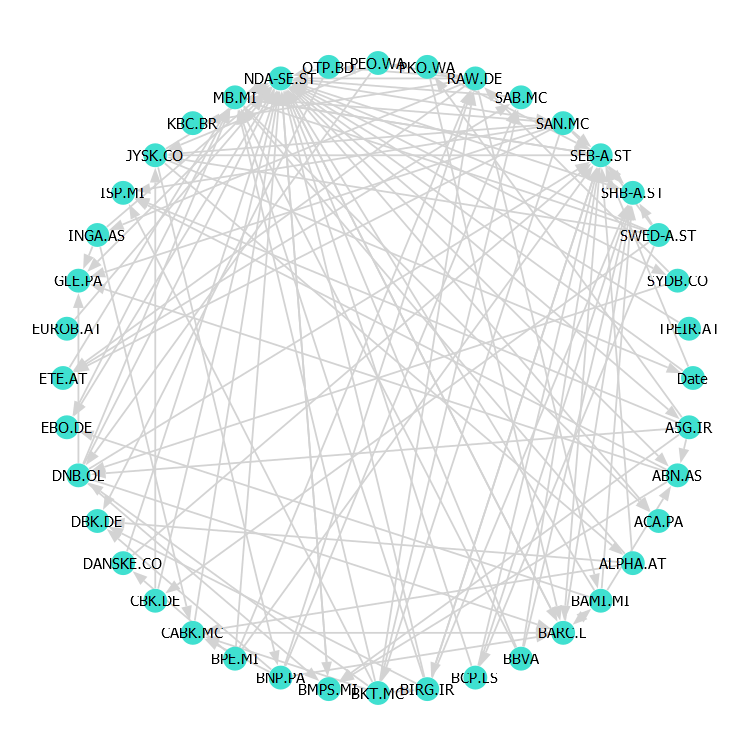
\includegraphics[width=7cm, height=7cm]{img/graph_eu_circl.png} }}
	\quad
	\subfloat[\centering Circle representation of graph]{{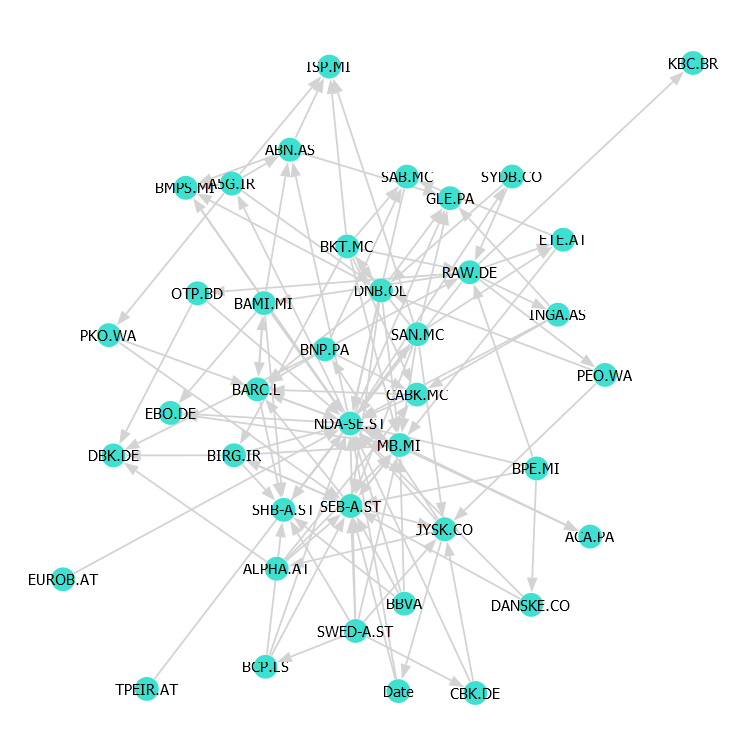
\includegraphics[width=7cm, height=7cm]{img/graph_eu.png} }}\\
	
	%	\subfloat[\centering Representation with random position]{{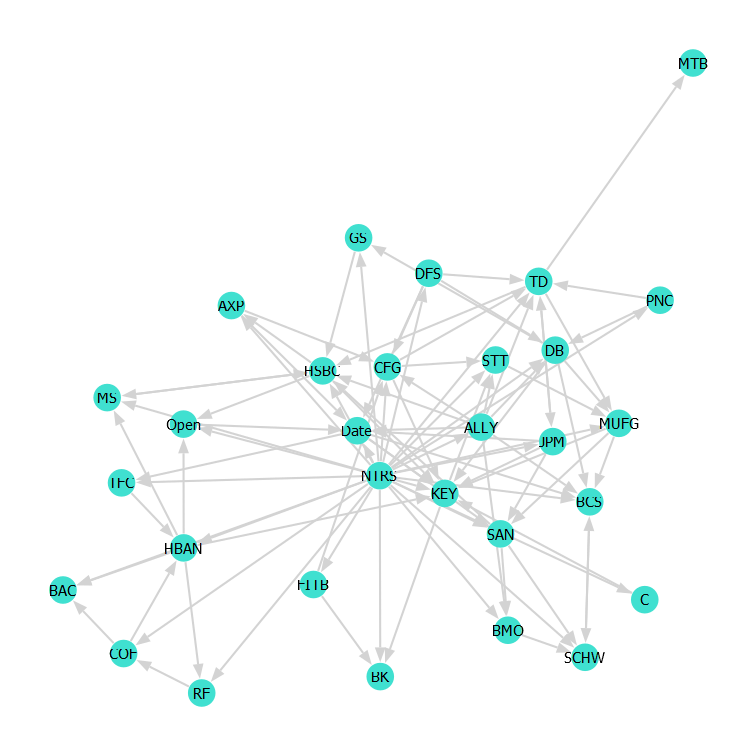
\includegraphics[width=7cm, height=7cm]{img/graph_us.png} }}
	%	\quad	
	%	\subfloat[\centering Circle representation of graph]{{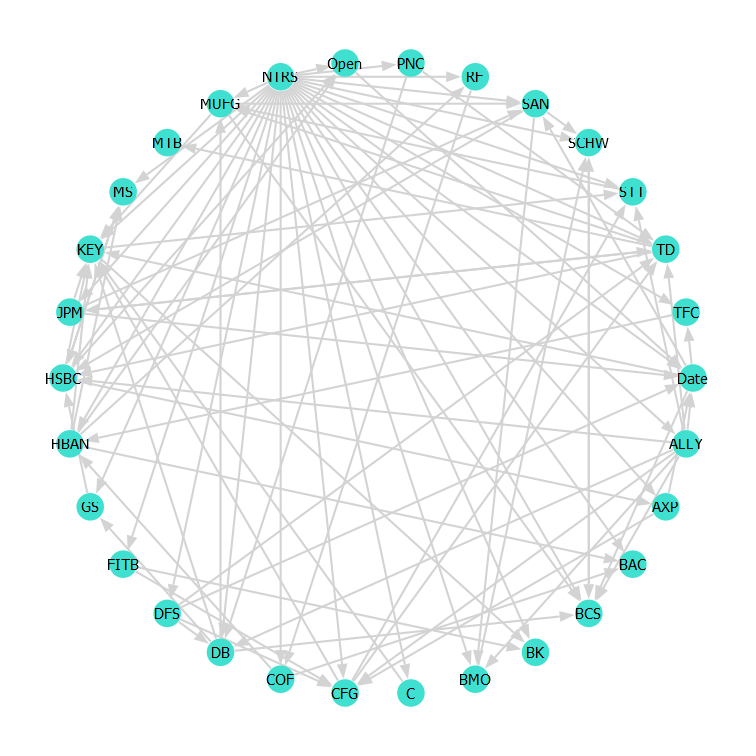
\includegraphics[width=7cm, height=7cm]{img/graph_us_circl.png} }}
	
	\caption{Financial network visualization based on the European market data from 2023. Each point (node) represents a financial institution and the connections (edges) are links estimated with the Granger causality method. The arrows indicate the direction of particular link. Each node is labeled with the ticker of given financial institution.}	\label{fig:actual_network}
\end{figure}


The literature investigating the topological nature of the interbank market often provide evidence of the \textit{dis-assortative} property of the network. In graph theory, the term assortativity refers to the tendency of nodes to be connected with the nodes of similar characteristic. In the context of financial networks, the term of \textit{dis-assortative} property is often used with respect to different bank features. For example, Based on the Brazilian interbank market, \cite{silva16} report its dis-assortative property with respect to the amount of connections of institutions\footnote{A similar reference is used e.g. in \cite{aldasoro17}} (node degree). The same property was observed on the Italian interbank market (\cite{bargigli15}). On the other hand, \cite{craig14} also provides evidence of dis-assortative behavior, however in this case, with respect to the bank size (i.e. smaller banks are more likely to be connected to the big ones).

\begin{table}
	\center
	\begin{tabular}{lcc c cc}
		\hline
		& \multicolumn{2}{c}{2023} & \multicolumn{2}{c}{2006}\\
		\cline{2-3} \cline{5-6} 
		\multicolumn{1}{l}{Network measures} & \multicolumn{1}{c}{Europe} & \multicolumn{1}{c}{US} && \multicolumn{1}{c}{US} & \multicolumn{1}{c}{Europe}\\
		\hline
		density & 0.0756 & 0.108 && 0.186 & 0.130 \\
		Average degree & 6.048 & 6.26 && 9.3 & 9.11 \\
		Median degree & 4 & 5 && 8 & 9 \\
		Excess degree assortativity & -0.373 & -0.324 && -0.324 & -0.245 \\
		Indegree assortativity & -0.188 & 0.137 && 0.1 & 0.162 \\
		Outderee assortativity & -0.31 & -0.0037 && -0.072 & 0.134 \\    
		Total degree assortativity & -0.2626 & -0.287 && -0.307 & -0.118 \\
		Cluster coefficient & 0.033 & 0.0459 && 0.078 & 0.053 \\
		intermediator share & 0.68 & 0.866 && 0.769 & 0.88 \\   
		Max path & 6 & 11 && 5 & 7 \\
		Relative max eigenvector centrality & 0.064 &  0.354 &&     0.221 & 0.163 \\
		Relative core size & 0.195 & 0.195 && 0.243 & 0.243 \\
		Absolute core size & 8 & 8 && 10 & 10 \\
		\hline
	\end{tabular}\
	\caption{Descriptive statistics of estimated networks. The definitions of each are described in appendix \ref{appendix:network_metrics}.}
	\label{table:network_metrics}
\end{table}

The assortativity, describing the correlation of node in/out-degree, is negative in almost every subsample of estimated networks, that is, they present a dis-assortative properties with respect to its degree. The only type of assortativity that is mostly positive is the indegree assortativity (measuring the correlation between the indegree of the connected nodes). It's worth to note, that the same pattern is present in some of the theoretical models (i.e. \cite{aldasoro17}). The negative values are expected. This is because the economic role of the interbank market is mostly to facilitate the flow of funds from banks with excess liquidity to those of funding needs. Thus, the banks are more likely connected with each other if their connections have, in overall, different directions of edges. As mentioned before, the empirical literature also reports mostly negative assortativity values.

The dis-assortative property of the financial network is a closely related  with the the \textit{core-periphery} structure of the network (\cite{craig14}). This structure is commonly observed in the transaction level data of the interbank market and is a widely acknowledged stylized fact. The structure is present when there is a core of the network with (usually bigger) banks, intermediating the flow of funds among the smaller ones. The banks tend to trade between the core and a periphery, but not within those groups. The identified core of the structure is rather stable between the financial markets but changes a bit throughout time. Nevertheless, the relative size is considerably higher than the estimates from the literature. For example, the seminal paper (\cite{craig14}) identifying the structure reports its relative size to be 3\% (depending on the specification). The reason for such a wide difference is most likely due to the sample used. This works mostly uses data of global systematically important institutions, which are most likely part of the core of the financial network. Another factor might be the different methodology applied to identify the core-periphery structure and the network itself. 

\subsection{Dynamic connectedness}

As mentioned before, the connectedness measure described in the section 
\ref{section:fin_network} are calculated in a rolling window bases. That is, at each time $t$ the connectedness is calculated for the past window of observations up to $t - w$, where $w$ is a window length. The calculations are done with two window lengths of a quarter and a year. The resulting time series from the calculation are presented in figure \ref{figure:connect_ts}. The variables were standardized ($\frac{x - \bar{x}}{\sigma_{x}}$), in order to be comparable among each other (also during the modeling stage).

\begin{figure}
	\centering
	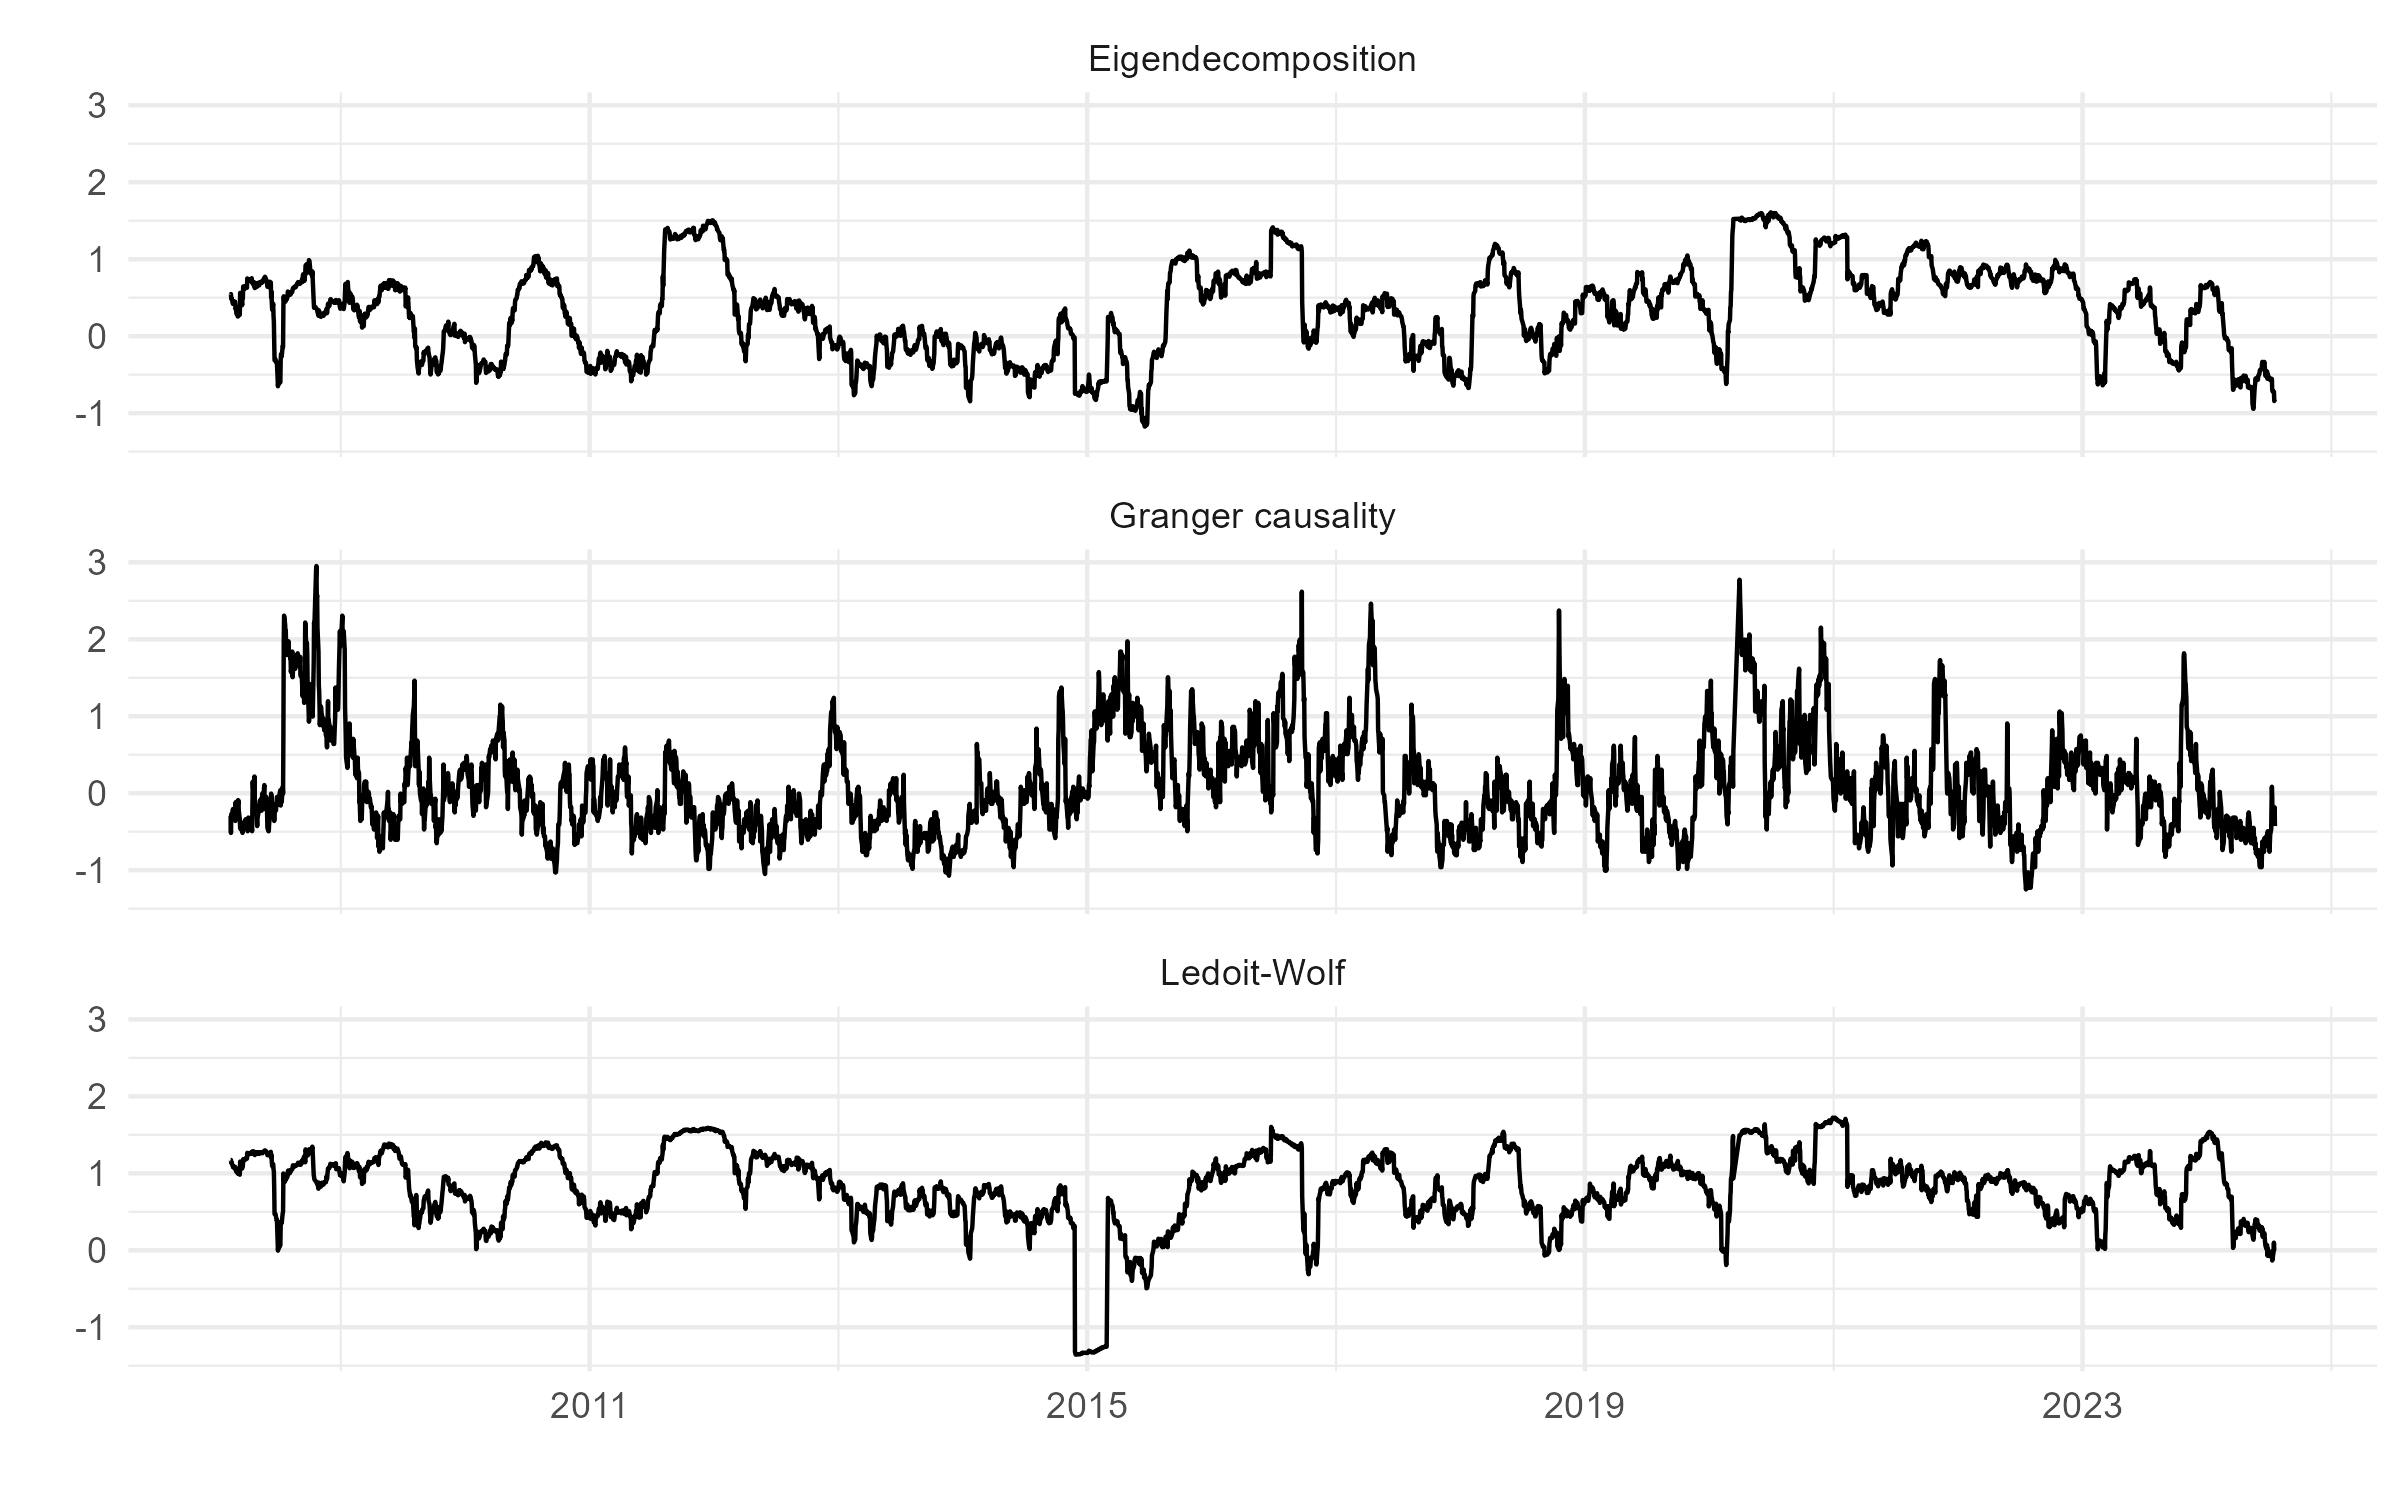
\includegraphics[scale = 0.76]{img/connect_ts.png}
	\caption{Connectedness time series of the US market. Rolling window of a quarter.}
	\label{figure:connect_ts}
\end{figure}

The Granger based method provides the most distinct and volatile time series. The method also captures a different type of connectedness. As noted already, it controls for the common exposures by introducing sectoral controls in the Granger regression. The other approaches are not controling for exogenous variables (other than subtracting the banking index returns) and are as well capturing linear relationship between the rates of return. The similarity is also confirmed by the Pearson's correlation equal to 77\% among the eigendecomposition and Ledoit-Wolf methods. On the other hand the Granger based connectedness time series has only 15\% and 3\% correlation with respect to the eigendecomposition and Ledoit-Wolf methods respectively\footnote{The full correlation matrix is shown on the figure \ref{figure:cor_matrix} in the appendix \ref{appendix:graphs_tables}.}.

\section{Regime-dependent effect of connectedness}

The previous section described in detail the methods of estimating the connectedness of the financial system. Subsequently, the resulting time series of the connectedness of the system are going to be utilized in the next process of time-series modeling. As the theoretical contribution posits, the connectedness should have a regime-dependent effect on the systemic stability of the financial sector. Thus, the econometric tool of choice is the Markov switching autoregressive conditional heteroskedasticity (ARCH) model. The class of models with Markov switching parameters were first proposed in the seminal work of \citet{hamilton89}, with the natural extension for ARCH effect in \citet{cai94}. Since then, these models were the go-to approach to model a time-variation and regime-change in the regression model parameters. 

As in usual process of ARCH modeling, the model requires to specify the mean equation:

\begin{equation}
	r_{b,t} = \beta_0 + \beta_1 r_{b_t-1} + \beta_2 r_{m, t-1} + \epsilon_t	
\end{equation}

Where $r_{b,t}$ and $r_{m, t}$ are rates of returns for banking index and broad market at time $t$ respectively. Subsequently, the absolute values of the residual are modeled with a regime-switching model:

\begin{equation}
	\sqrt{\epsilon^{2}_t} = \alpha_{0,S_t} + \underbrace{\alpha_{1,S_t} \gamma_{t-1}}_{\text{connectedness}} + \underbrace{\sum_{i=1}^{p} \alpha_{i+1} \sqrt{\epsilon^2_{t-i}}}_{\text{lag controls}}
\end{equation}

Where $\gamma_t$ is, as before, the financial connectedness at time $t$\footnote{Of course, there are different connectedness variables, calculated with different methods, rolling window sizes and markets but the indices are omitted for the sake of brevity.}. The lag covariates control for the heteroskedasticity, common in financial time-series. An important assumption in the model is that the volatility (or the absolute rates of return) of the banking index is the appropriate proxy for the stability of the financial sector. There are some theoretical arguments that it may not always be the case (see e.g. the literature regarding the volatility paradox - \citet{brunnermeier14} or \citet{danielsson18}), nonetheless it is still a commonly utilized proxy in the literature (some of the examples are \citet{nelson07}, \citet{bratis20}, \citet{imf08} or \citet{billio16}).

The $\gamma_{t-1}$ and the corresponding coefficient $\alpha_{1, S_t}$ are the relevant term of interest to the research design. Notably, the connectedness time series is lagged by a single period. This operation is subtle yet crucial, as the instantaneous relationship between the system stability and connectedness may not be fully exogenous. The connectedness measures, especially the one based on Ledoit-Wolf estimation, are still imperfect estimations and captures to some degree a simple correlation among the stock returns. It is commonly acknowledged that the correlations increases also as a consequence of sudden volatility spikes. For example, due to the margin calls (\citet{kahraman19}) or fly to safety effects (\citet{baele19}). Additionally, the banks themselves may make hedging decision in the face of market uncertainty, thus changing the connections among each other. In order to eliminate this source of endogeneity, the connectedness variables are lagged by a single period. With this specification, the model investigates how the financial stability evolves under different connectedness levels prior to the arrival of the shock. Because of this, the coefficient have a causal interpretation. 

The parameters indexed by $S_t$ depends upon the latent (unobservable) state, that may take values from 1 to $K$. The parameters change their values depending on the state. The state $K$ is governed by the Markov process. The probability of transition from state $i$ to state $j$ is given by $K \times K$ left-stochastic transition matrix $\mathbf{P}$:

\begin{equation}
	\mathbf{P} = P(S_t = i | S_{t-1} = j) = 
	\begin{bmatrix}
		\pi_{1,1} & \pi_{1,2} & \cdots & \pi_{1,k} \\
		\pi_{2,1} & \pi_{2,2} & \cdots & \pi_{2,k} \\
		\vdots  & \vdots  & \ddots & \vdots  \\
		\pi_{k,1} & \pi_{k,2} & \cdots & \pi_{k,k} 
	\end{bmatrix}
\end{equation}

With standard constraints $\sum_{i}^{K} \pi_{i,j} = 1 \; \forall j \in \{1,\cdot, K\}$ and $0 \geq \pi_{i,j} \geq 1 \; \forall i,j \in \{1,\cdot, K\}$. For the state size $K=2$, which is the case for herein model, the constraint for the transition matrix may be easily imposed with following parametrization:

\begin{equation}
	P(S_t = i | S_{t-1} = j) = \begin{bmatrix}
		\pi_1 & 1 - \pi_2\\
		1 - \pi_1 & \pi_2
	\end{bmatrix}
\end{equation}



\bibliography{bibliography}

\newpage

\appendix

\section{Data}\label{appendix:data}

\begin{table}[!htbp]
	\begin{center}
		\renewcommand{\arraystretch}{0.8}
		\resizebox{\textwidth}{!}{\begin{tabular}{c|c||c |c|c}\multicolumn{2}{c||}{USA} & \multicolumn{2}{c}{EU} \\
			\hline \hline 
			Ticker & Name & Ticker & Name & Country \\
			\hline \hline
			BAC & Bank of America Corporation & EBO & Erste Group Bank AG & Austria \\
			\hline
			BK & The Bank of New York Mellon & RAW & Raiffeisen Bank AG & Austria\\
			\hline
			BCS & Barclays* & KBC & KBC Group & Belgium\\
			\hline
			BMO & Bank of Montreal* & CBK & Commerzbank AG & Germany \\
			\hline
			COF & Capital One Financial Corporation & DBK & Deutsche Bank AG & Germany \\
			\hline
			SCHW & The Charles Schwab Corporation & NDA-SE & Nordea & Finland \\
			\hline
			C & Citigroup & DANSKE & Danske Bank A/S & Denmark \\
			\hline
			CFG & Citizens Financial Group & JYSK & Jyske Bank A/S & Denmark \\
			\hline
			DB & Deutsche Bank* & SYDB & Sydbank A/S & Denmark \\
			\hline
			GS & The Goldman Sachs Group & BBVA & Banco Bilbao Vizcaya & Spain \\
			\hline
			JPM & JPMorgan Chase \& Co. & BKT & Bankinter SA & Spain \\
			\hline
			MTB & M\&T Bank Corporation & CABK & CaixaBank SA & Spain \\
			\hline
			MS & Morgan Stanley & SAB & Banco de Sabadell SA & Spain \\
			\hline
			NTRS & Northern Trust Corporation & SAN & Banco Santander SA & Spain \\
			\hline
			PNC & The PNC Financial Services Group & UNI & Unicaja Banco SA & Spain \\
			\hline
			STT & State Street Corporation & BNP &  BNP Paribas SA & France \\
			\hline
			TD & The Toronto Dominion Bank* & ACA & Crédit Agricole SA & France \\
			\hline
			TFC & Truist Financial Corporation & GLE & Société Générale & France \\
			\hline
			UBS & UBS Group AG* & ALPHA & Alpha Services and Holdings SA & Greece \\
			\hline
			WFC & Wells Fargo \& Company & EUROB & Eurobank Ergasias & Greece \\
			\hline
			ALLY & Ally Financial Inc. & ETE & National Bank of Greece SA & Greece \\
			\hline
			AXP & American Express Company & TPEIR & Piraeus Financial Holdings SA & Greece \\
			\hline
			DFS & Discover Financial Services & OTP & OTP Bank Nyrt & Hungary \\
			\hline
			FITB & Fifth Third Bancorp & A5G & AIB Group plc & Ireland \\
			\hline
			HSBC & HSBC Holdings plc* & BARC & Barclays PLC & Great Britain \\
			\hline
			HBAN & Huntington Bancshares Incorporated & BARC & Barclays PLC & Great Britain \\
			\hline
			KEY & KeyCorp Bank & BIRG & Bank of Ireland Group & Ireland \\
			\hline
			MUFG & Mitsubishi UFJ Financial Group* & BAMI & Banco BPM S.p.A. & Italy \\
			\hline 
			PNC & The PNC Financial Services Group & ISP & Intesa Sanpaolo S.p.A. & Italy \\
			\hline
			RF & Regions Financial Corporation & MB & Mediobanca Banca di Credito Finanziario S.p.A. & Italy \\
			\hline
			SAN & Banco Santander, S.A.* & BMPS & Banca Monte dei Paschi di Siena S.p.A. & Italy \\
			\hline
			& & BPE & BPER Banca S.p.A. & Italy \\
			\hline
			& & UCG & UniCredit S.p.A. & Italy \\
			\hline
			& & ABN & ABN AMRO Bank N.V. & Netherlands \\
			\hline
			& & INGA & ING Groep N.V. & Netherlands \\
			\hline
			& & DNB & DNB Bank ASA & Norway \\
			\hline
			& & PKO & Powszechna Kasa Oszczednosci Bank Polski S.A. & Poland \\
			\hline
			& & PEO & Bank Polska Kasa Opieki S.A. & Poland \\
			\hline
			& & BCP & Banco Comercial Português S.A. & Portugal \\
			\hline
			& & SEB-A & Skandinaviska Enskilda Banken AB & Sweden \\
			\hline
			& & SHB-A & Svenska Handelsbanken AB & Sweden \\
			\hline
			& & SWED-A & Swedbank AB & Sweden
		\end{tabular}}
	\end{center}
	\caption{List of the banks analyzed. *These banks are not registered in USA but are apparently systematically important to the local market according to the regulator. }
	\label{table:bank_list}
\end{table}

% latex table generated in R 4.3.2 by xtable 1.8-4 package
% Sat Jul 20 14:54:42 2024
\begin{table}[!htbp]
	\centering
	\renewcommand{\arraystretch}{0.7}
	\begin{tabular}{l|l|l|l}\multicolumn{2}{c|}{USA} & \multicolumn{2}{c}{EU} \\
		\hline
		Ticker & IPO date & Ticker & IPO date \\ 
		\hline 
		ALLY & 2014-01-29 & A5G & 2000-01-06 \\ 
		AXP & 2000-01-06 & ABN & 2015-11-23 \\ 
		BAC & 2000-01-06 & ACA & 2001-12-17 \\ 
		BCS & 2000-01-06 & ALPHA & 2000-01-06 \\ 
		BK & 2000-01-06 & BAMI & 2000-01-06 \\ 
		BMO & 2000-01-06 & BARC & 2000-01-06 \\ 
		C & 2000-01-06 & BBVA & 2000-01-06 \\ 
		CFG & 2014-09-25 & BCP & 2000-01-06 \\ 
		COF & 2000-01-06 & BIRG & 2001-07-16 \\ 
		DB & 2000-01-06 & BKT & 2000-01-06 \\ 
		DFS & 2007-06-15 & BMPS & 2000-01-06 \\ 
		FITB & 2000-01-06 & BNP & 2000-01-06 \\ 
		GS & 2000-01-06 & BPE & 2000-01-06 \\ 
		HBAN & 2000-01-06 & CABK & 2007-10-11 \\ 
		HSBC & 2000-01-06 & CBK & 2000-01-06 \\ 
		JPM & 2000-01-06 & DANSKE & 2000-11-09 \\ 
		KEY & 2000-01-06 & DBK & 2000-01-06 \\ 
		MS & 2000-01-06 & DNB & 2000-01-06 \\ 
		MTB & 2000-01-06 & EBO & 2009-03-31 \\ 
		MUFG & 2001-04-03 & ETE & 2000-01-06 \\ 
		NTRS & 2000-01-06 & EUROB & 2000-01-06 \\ 
		Open & 2000-01-06 & GLE & 2000-01-06 \\ 
		PNC & 2000-01-06 & INGA & 2000-01-06 \\ 
		RF & 2000-01-06 & ISP & 2000-01-06 \\ 
		SAN & 2000-01-06 & JYSK & 2004-10-05 \\ 
		SCHW & 2000-01-06 & KBC & 2000-01-06 \\ 
		STT & 2000-01-06 & MB & 2000-01-06 \\ 
		TD & 2000-01-06 & NDA & 2000-01-06 \\ 
		TFC & 2000-01-06 & OTP & 2002-03-06 \\ 
		UBS & 2000-05-17 & PEO & 2000-01-06 \\ 
		&  & PKO & 2004-11-11 \\ 
		&  & RAW & 2010-08-17 \\ 
		&  & SAB & 2000-01-06 \\ 
		&  & SAN & 2000-01-06 \\ 
		&  & SEB & 2000-01-06 \\ 
		&  & SHB & 2000-01-06 \\ 
		&  & SWED & 2000-01-06 \\ 
		&  & SYDB & 2000-01-06 \\ 
		&  & TPEIR & 2000-01-06 \\ 
		&  & UCG & 2000-01-06 \\ 
		&  & UNI & 2017-07-03 
	\end{tabular}
		\caption{First available data for each of the stock prices. }
	\label{table:ipo}
\end{table}

\section{Network metrics}\label{appendix:network_metrics}

We define a graph $G = (V, E)$ to be an abstract object with a set of $E$ edges (or links) and a set of $V$ vertices (or nodes). The nodes are connected with edges in a graph. The node set $V$ and a set of edges $E$ is denoted as $V(G)$ and $E(G)$. The cardinality of these sets are usually denoted as $m = |E|$ for edges and $n = |V|$ for nodes. The edges may be represented by the nodes they connect - $(u, v)$ (or with shorthand notation $uv$). In case of directed graph, the order of the notation matters, as it defines the direction of the edge ($uv \neq vu$). For the weighted graph, the values associated to the nodes may be represented as a function $\omega : E \rightarrow \mathcal{R}$, assigning each edge $e \in E$ a weight $\omega(e)$. In case of the financial networks, the values may describe e.g. the exposure of the bilateral contractual obligation between the financial intermediaries. The undirected graphs are equivalent to the weighted ones with a unit edge weights $\omega(e) = 1 \; \forall \; e \in E$.

Degree, denoted as $d(v)$ is the number of edges of particular node $v$. For a directed graph, the \textit{out-degree} of $v \in V$ is denoted as $d^{+}(v)$, define the number of edges with the origin $v$. Analogically, the \textit{in-degree} is denoted as $d^{-}(v)$ is the number of the edges with destination at $v$.

As mentioned in the subsection $\ref{section:fin_network}$, the graph theory has a very appealing relation to the linear algebra. Every graph may be represented by its adjacency matrix, often denoted $\mathbf{A}$. In case of unweighted, directed graph, the adjacency matrix has values $a_{i,j} \in \{0,1\}$, indicating a node connection. That is, $a_{i,j} = 1 \Rightarrow i \rightarrow j \; \forall \;  i \neq j$. The matrix elements may take other values in case of the weighted graph. 

\subsection{Graph statistics definition}

\textbf{Network density} measures the connectedness of the network. The statistic is defined as:

\begin{equation}
	\gamma(G) \coloneqq \frac{m}{{n \choose 2}}
\end{equation}

\textbf{Average degree} is simply the average number of edges for each of the node in the graph:

\begin{equation}
	\bar{d}(G) = \frac{1}{n} \sum_{v \in V} d(v)
\end{equation}

The \textbf{median degree} is defined in a corresponding fashion.

The \textbf{assortativity} measures the correlation among the connected nodes with respect to their characteristics. It's calculation follows the Pearson correlation coefficient:

\begin{equation}
	r(G) = \frac{\sum_{uv \in E}^{m} (d(u) - \bar{d}(G)) (d(v) - \bar{d}(G))}{\sqrt{\sum_{uv \in E}^{m} (d(u) - \bar{d}(G))^2} \sqrt{\sum_{uv \in E}^{m} (d(v) - \bar{d}(G))^2}} \;, E \in G
\end{equation}

Naturally, as for the Pearson's correlation, it takes values between -1 and 1 and is interpreted in the same way as well. Depending on type of the assortativity, the correlation may be calculated based on other measure than degree of the node ($d(u)$). The excess degree assortativity is defined as in \cite{newman02} and uses outdegree value for source node $u$ and indegree for destination node $v$.

The \textbf{clustering coefficient} measure the relative amount of clusters. It is calculated as a share of closed triplets in total number of possible triplets of the graph. The closed triplet, being a three connected nodes. The calculation is easily defined with a matrix notation:

\begin{equation}
	C(\mathbf{A}) = \frac{\sum_{i}^{n} \sum_{j}^{n} \sum_{k}^{n} a_{i,j} a_{j,k} a_{k,i}}{\frac{1}{2} \sum_{i}^{n} k_i (k_i - 1)}
\end{equation}

Where $k_i = \sum_{j}^{n} a_{i,j}$. 

The \textbf{intermediator share} is simply a share of nodes with both indegree and outdegree:

\begin{equation}
	\frac{1}{n} \sum_{v \in V}^{n} \min\{1, \, d^{+}(v) d^{-}(v)\}
\end{equation}

The \textbf{maximum path} is the biggest set (in sense of cardinality) of distinct edges connecting nodes for every pair of the nodes. 

The \textbf{relative max eigenvector centrality} is a share of the node with the highest eigenvector centrality in the total sum of the centrality measures in the whole graph. The eigenvector centrality $c$ satisfies the following equation:

\begin{equation}
	\lambda c_i = \sum_{j \neq i}^{n} a_{j,i} c_j
\end{equation}

Or alternatively in the matrix formulation:

\begin{equation}
	\lambda \mathbf{c} = \mathbf{A}' \mathbf{c}
\end{equation}

The euqation may be solved as described in the subsection \ref{subsection:pca}. The appealing property of the measure is that the centrality of the node $i$ is proportional to the centrality of its directly neighboring nodes\footnote{It is clear when the change of the index of $c$ at the R.H.S. is spotted}. Additionally, the node may be central in the system either through the number of neighbors or the value of their centrality.

\subsection{Graphs and tables}\label{appendix:graphs_tables}

\begin{figure}[!htbp]
	\centering
	\subfloat[\centering Circle representation of graph]{{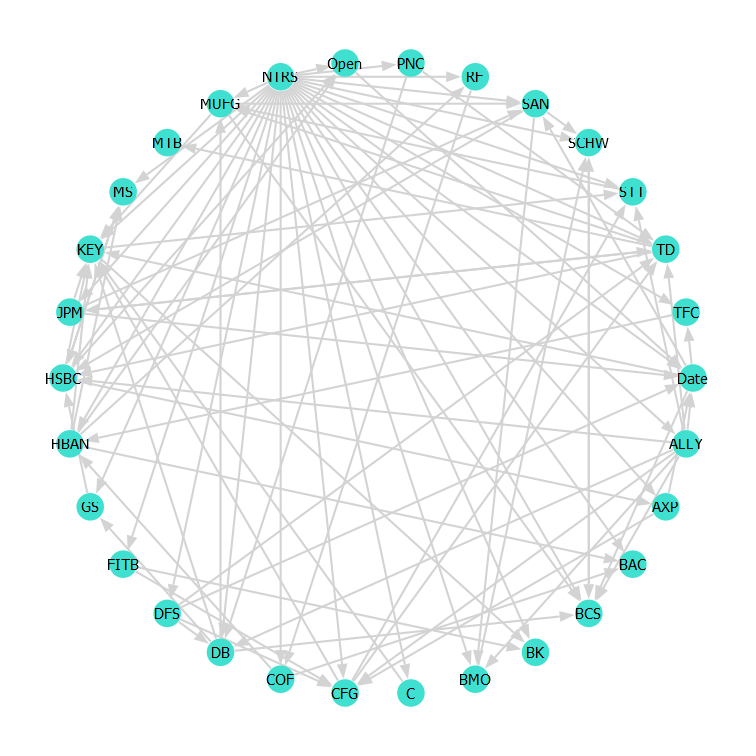
\includegraphics[width=7cm, height=7cm]{img/graph_us_circl.png} }}
	\quad
	\subfloat[\centering Circle representation of graph]{{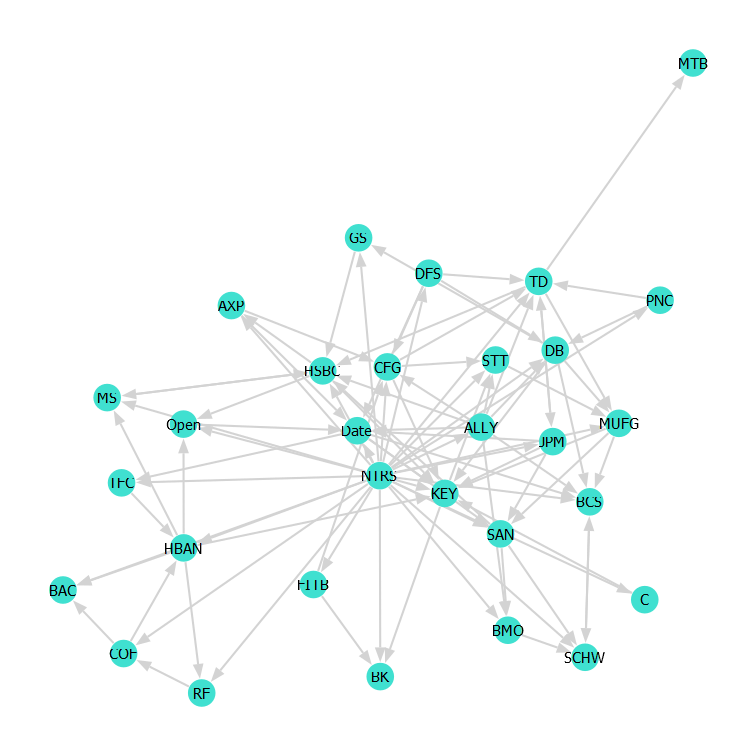
\includegraphics[width=7cm, height=7cm]{img/graph_us.png} }}\\
	
	%	\subfloat[\centering Representation with random position]{{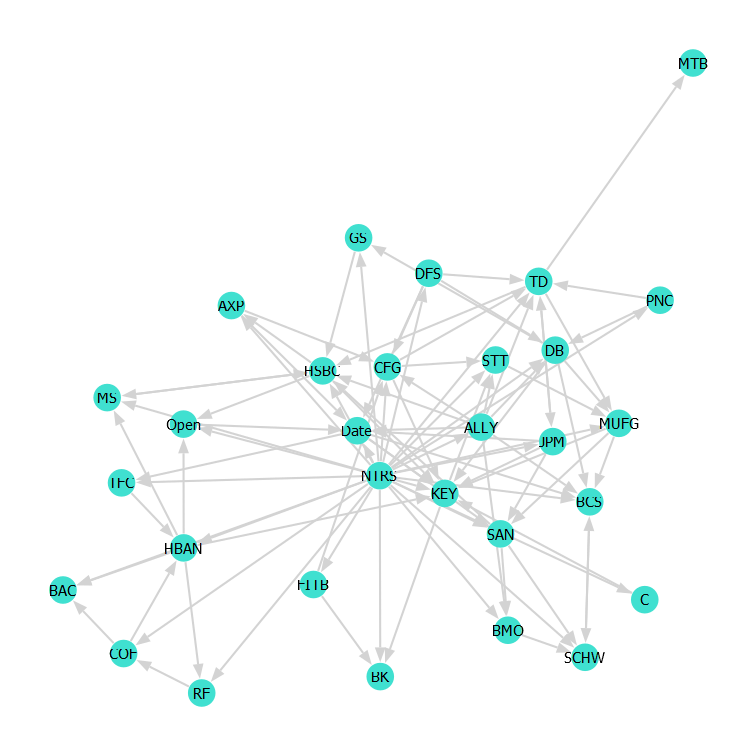
\includegraphics[width=7cm, height=7cm]{img/graph_us.png} }}
	%	\quad	
	%	\subfloat[\centering Circle representation of graph]{{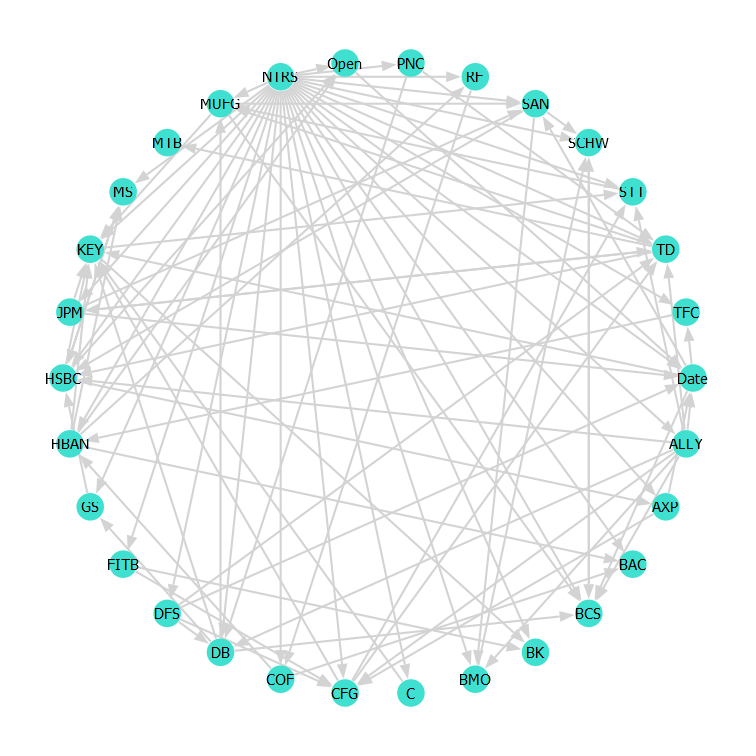
\includegraphics[width=7cm, height=7cm]{img/graph_us_circl.png} }}
	
	\caption{Financial network visualization based on the US market data from 2023. Each point (node) represents a financial institution and the connections (edges) are estimated links.}	\label{fig:actual_network}
\end{figure}

\begin{figure}[!htbp]
		\centering
	\subfloat[\centering Circle representation of EU financial network]{{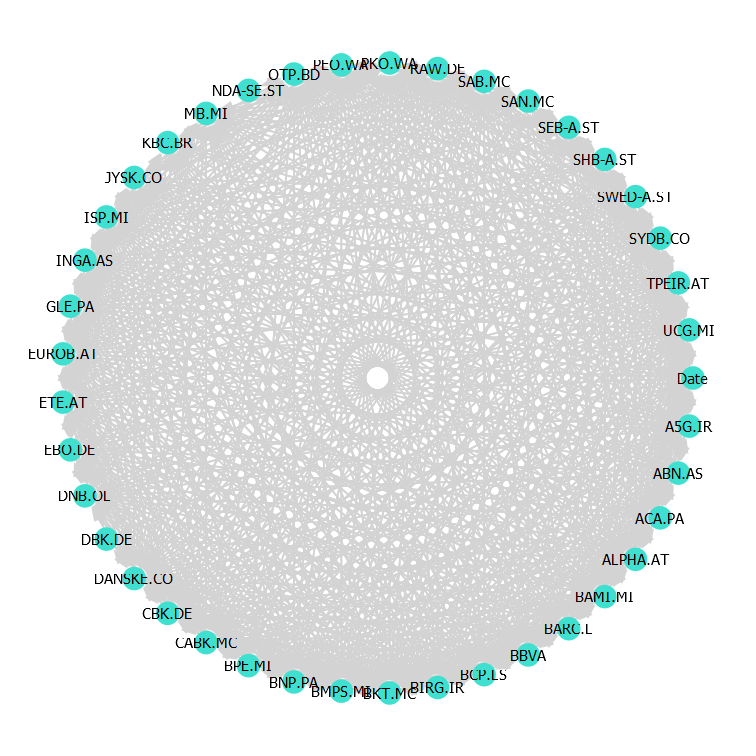
\includegraphics[width=7cm, height=7cm]{img/graph_eu_lw_circl.png} }}
	\quad
	\subfloat[\centering EU financial network representation with random position]{{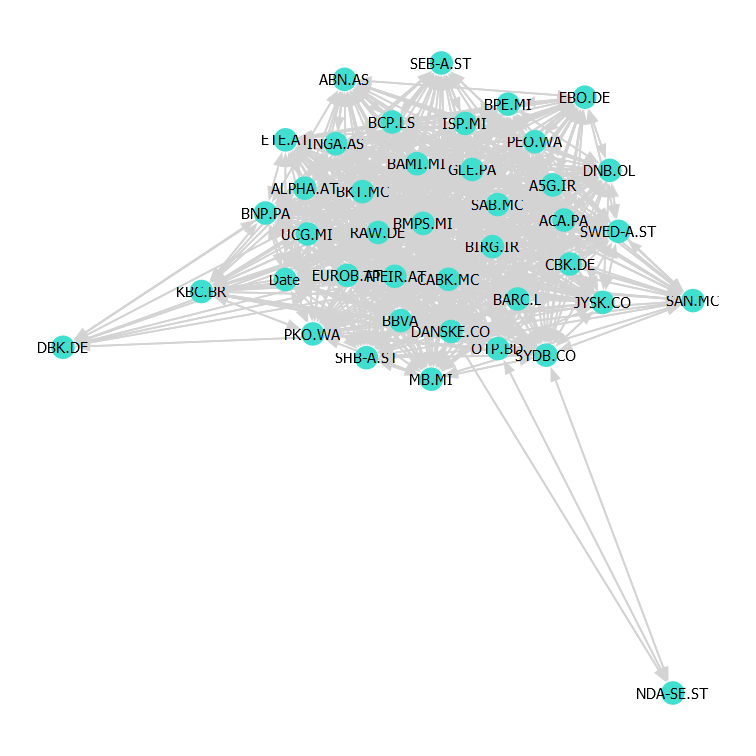
\includegraphics[width=7cm, height=7cm]{img/graph_eu_lw.png} }}\\
	
	\subfloat[\centering US financial network representation with random position]{{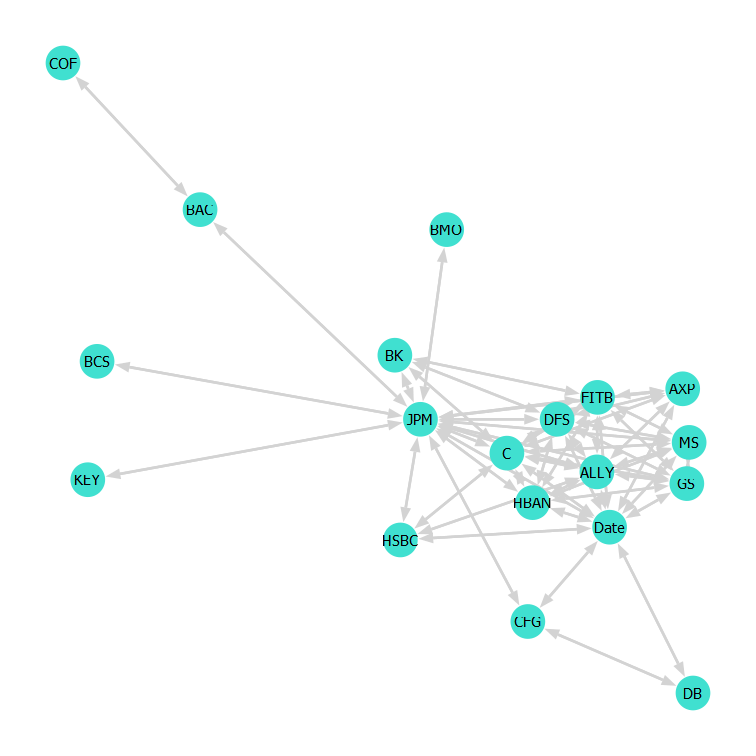
\includegraphics[width=7cm, height=7cm]{img/graph_us_lw.png} }}
	\quad	
	\subfloat[\centering Circle representation of US financial network]{{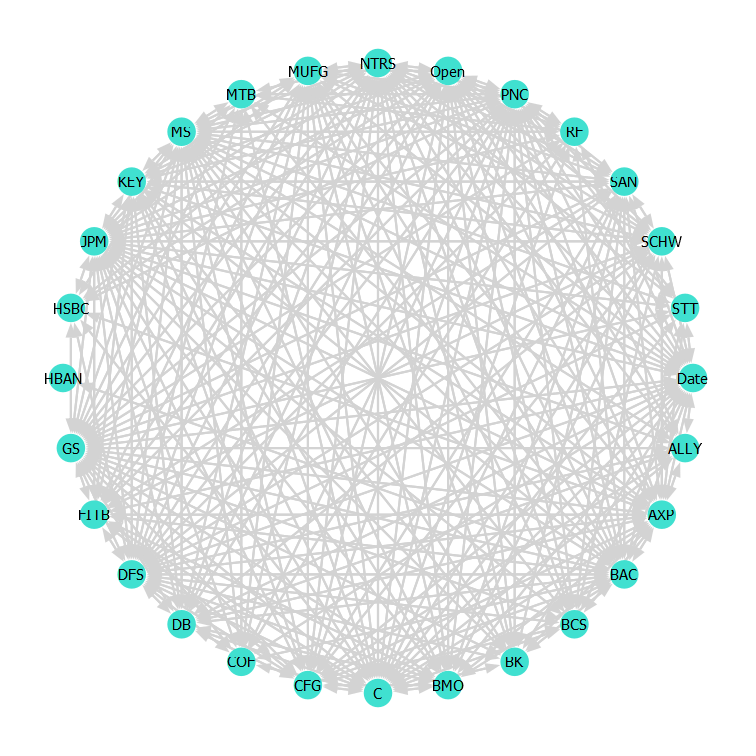
\includegraphics[width=7cm, height=7cm]{img/graph_us_lw_circl.png} }}
	
	\caption{Graph visualization based on the data from 2023. Each point (node) represents a financial institution and the connections (edges) are estimated links. The network is estimated with the Ledoit-Wolf covariance estimator. The nodes are assumed to be connected if the estimated covariance exceeds 0.02\%}	\label{fig:actual_network_lw}
\end{figure}

\begin{table}[!htbp]
	\center
	\begin{tabular}{l |c|c}
		Metric & EU & US \\
		\hline
		Density & 0.117 & 0.135 \\
		Average degree & 9.36 & 7.86 \\
		Median degree & 8 & 3 \\
		Assortativity & -0.485 & -0.372 \\
		Cluster coefficient & 0.105 & 0.162 \\
		Intermediator share & 0.682 & 0.633 \\
		Max path & 3 & 4 \\
		Eigenvector centrality & 0.109 & 0.121 \\
		Core size (\%) & 17.07 & 19.51 \\
		Absolute core size & 7 & 8 \\
	\end{tabular}
	\label{table:lw_stats}
	\caption{Network metrics of financial network estimated with Ledoit-Wolf shrinkage method. Data from 2023}
\end{table}

\begin{figure}
	\centering
	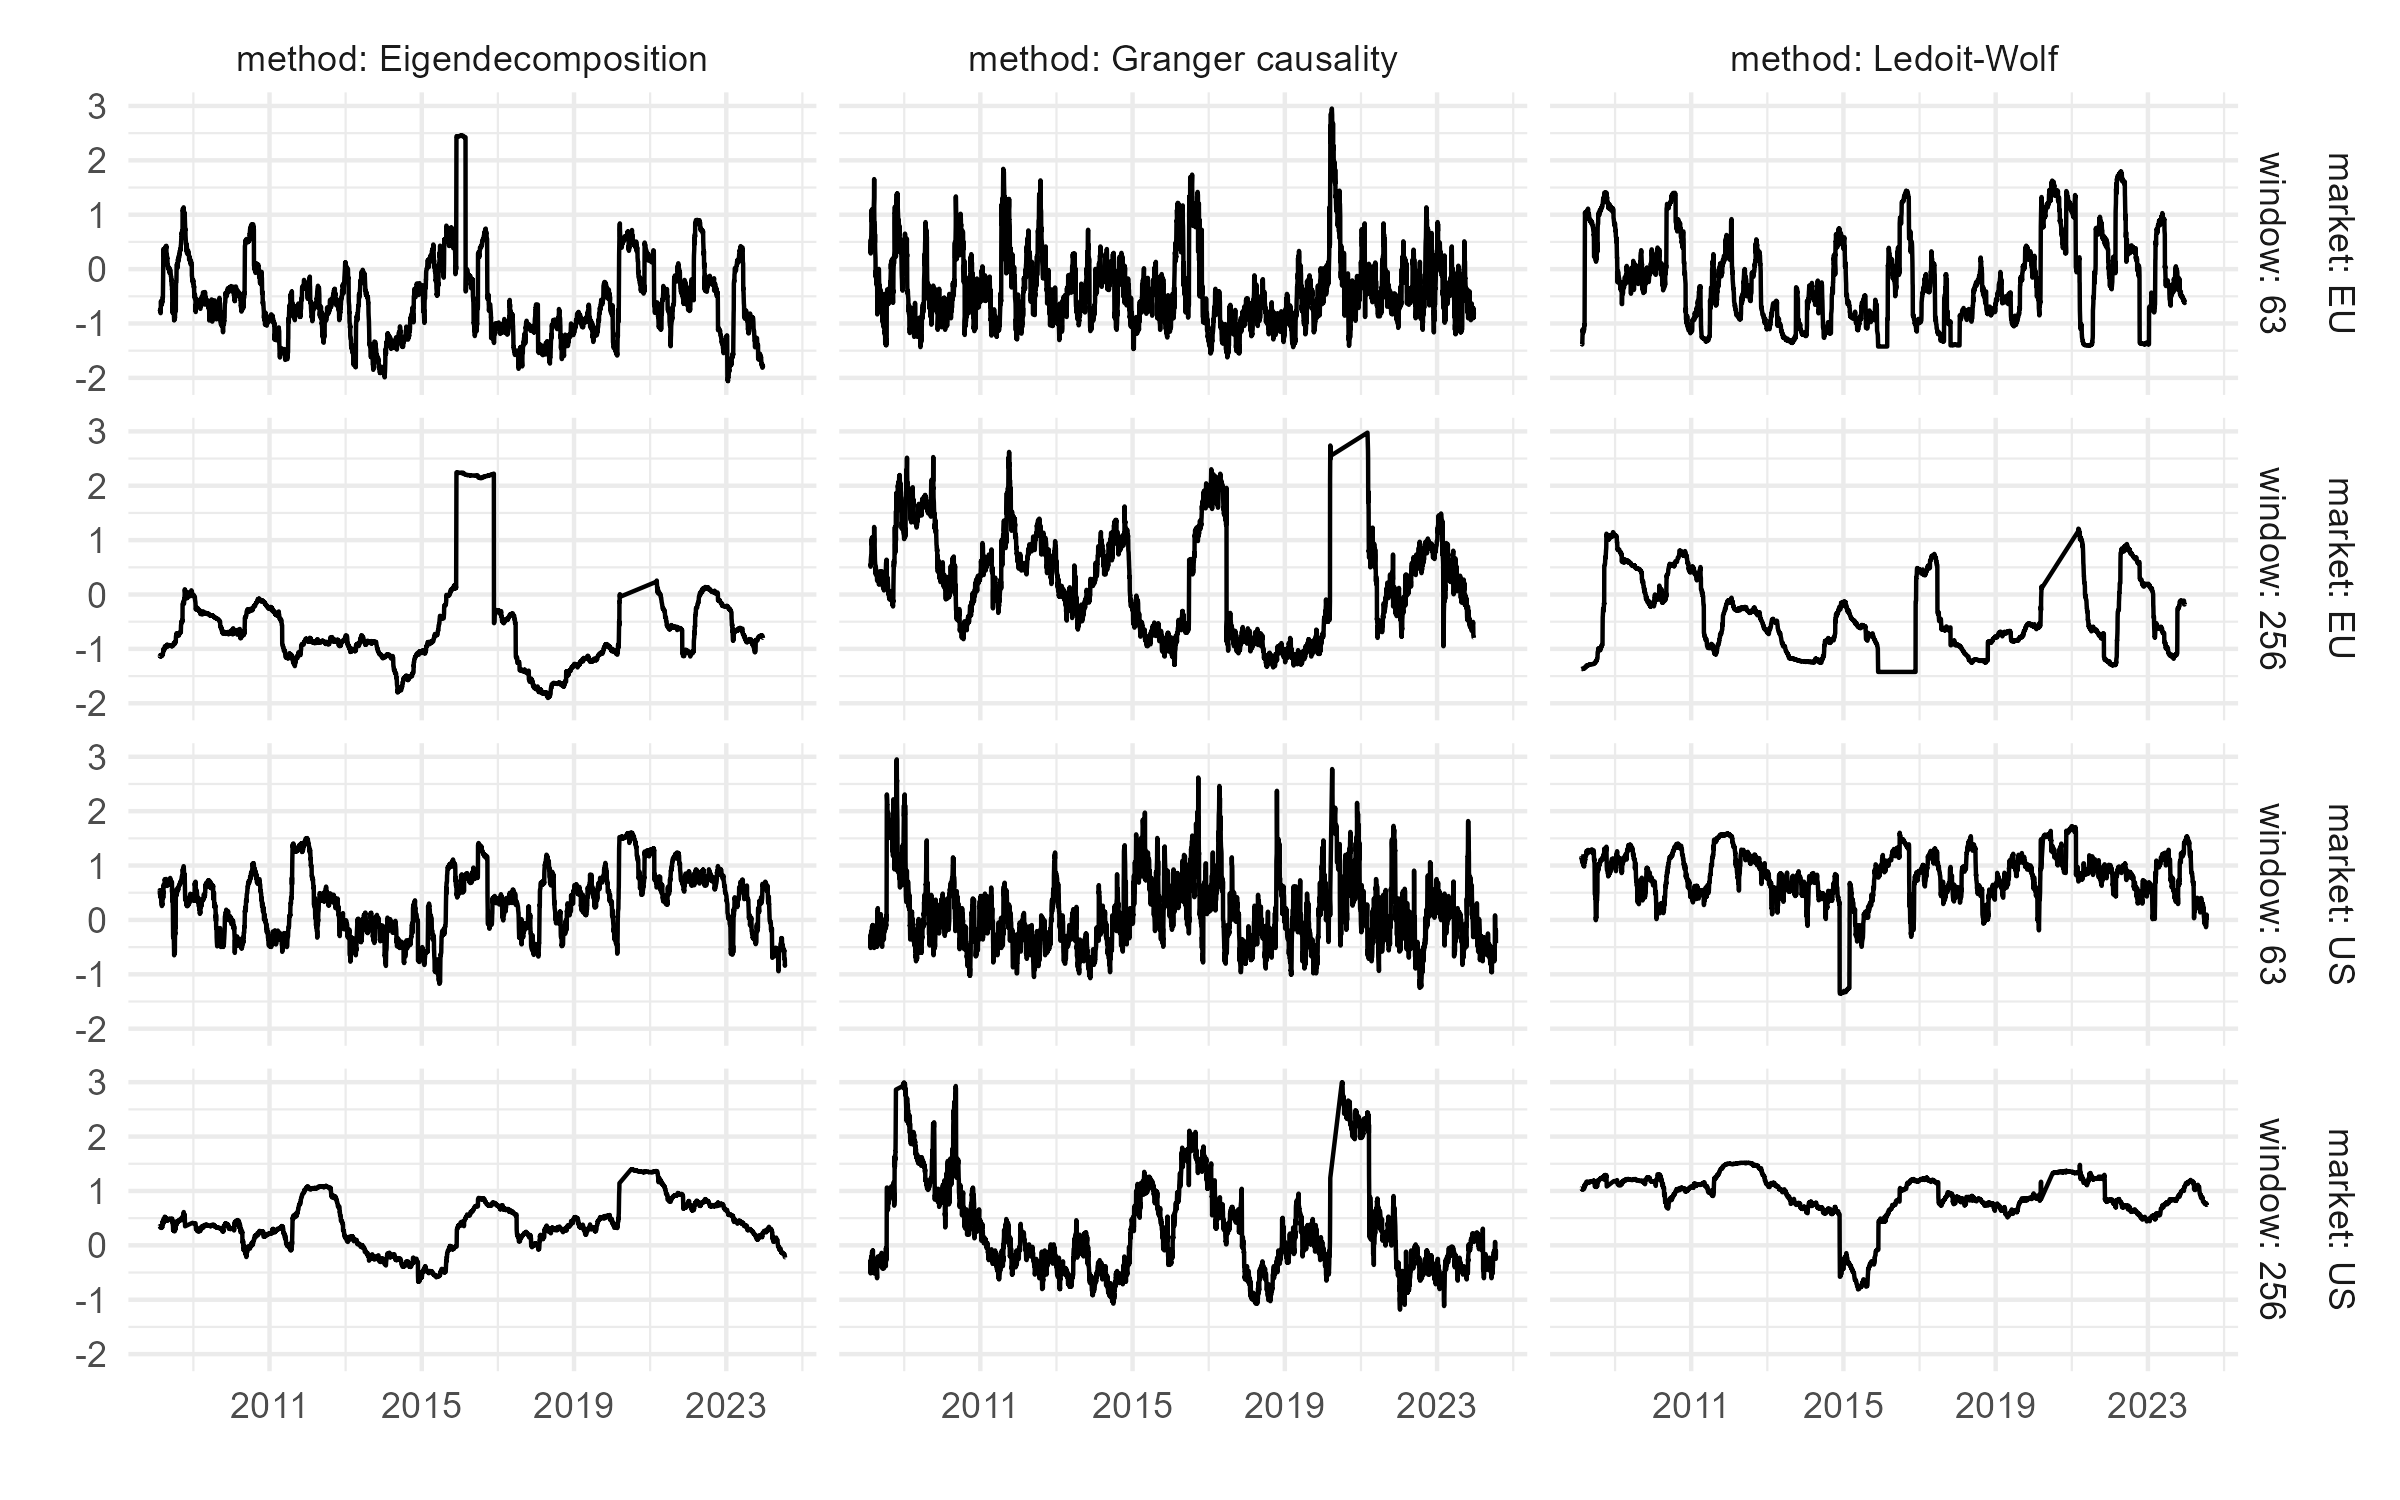
\includegraphics[scale = 0.8]{img/connect_ts_app.png}
	\caption{Connectedness time series}
	\label{figure:connect_ts_app}
\end{figure}

% latex table generated in R 4.3.2 by xtable 1.8-4 package
% Tue Aug  6 13:36:59 2024
% latex table generated in R 4.3.2 by xtable 1.8-4 package
% Tue Aug  6 13:44:42 2024
\begin{table}[ht]
	\centering
	\begin{tabular}{rrrrrrr}
		\hline
		& cor\_lw\_us\_256 & cor\_lw\_us\_63 & eig\_us\_256 & eig\_us\_63 & granger\_us\_256 & granger\_us\_63 \\ 
		\hline
		cor\_lw\_us\_256 & 1.00 & 0.59 & 0.65 & 0.29 & 0.12 & -0.15 \\ 
		cor\_lw\_us\_63 & 0.59 & 1.00 & 0.57 & 0.77 & 0.17 & 0.03 \\ 
		eig\_us\_256 & 0.65 & 0.57 & 1.00 & 0.66 & 0.28 & 0.07 \\ 
		eig\_us\_63 & 0.29 & 0.77 & 0.66 & 1.00 & 0.23 & 0.16 \\ 
		granger\_us\_256 & 0.12 & 0.17 & 0.28 & 0.23 & 1.00 & 0.45 \\ 
		granger\_us\_63 & -0.15 & 0.03 & 0.07 & 0.16 & 0.45 & 1.00 \\ 
		\hline
	\end{tabular}
		\caption{Pearson correlation matrix among the different specifications of connectedness time series}
		\label{figure:cor_matrix}
\end{table}

\end{document}